% !TeX program = xelatex
% 中文期刊论文：按照南方电网技术投稿要求改写
% 编译建议：XeLaTeX。中文字体优先使用系统字体，缺失时回退到 TeX Live/CTeX 常见的 Fandol 字体。
\documentclass[UTF8,zihao=5,twoside]{ctexart}

\usepackage[a4paper,top=22mm,bottom=20mm,left=18mm,right=18mm,headheight=14pt,headsep=6mm,columnsep=7mm]{geometry}
\usepackage{fontspec}
\usepackage{xeCJK}
\usepackage{amsmath,amssymb,bm}
\usepackage{graphicx}
\usepackage{float}
\usepackage{booktabs,array,multirow,tabularx}
\usepackage{caption}
\usepackage{titlesec}
\usepackage{fancyhdr}
\usepackage{indentfirst}
\usepackage{enumitem}
\usepackage{multicol}
\usepackage{balance}
\usepackage{tikz}
\usetikzlibrary{arrows.meta,positioning,shapes.geometric}
\usepackage[hidelinks]{hyperref}

\graphicspath{{figures/}}

% -------------------- 字体 --------------------
\IfFontExistsTF{Songti SC}
  {\setCJKmainfont{Songti SC}}
  {\IfFontExistsTF{SimSun}
    {\setCJKmainfont{SimSun}}
    {\setCJKmainfont{FandolSong-Regular.otf}[BoldFont=FandolSong-Bold.otf,ItalicFont=FandolKai-Regular.otf]}}
\IfFontExistsTF{Heiti SC}
  {\setCJKsansfont{Heiti SC}}
  {\IfFontExistsTF{SimHei}
    {\setCJKsansfont{SimHei}}
    {\setCJKsansfont{FandolHei-Regular.otf}[BoldFont=FandolHei-Bold.otf]}}
\IfFontExistsTF{Kaiti SC}
  {\setCJKfamilyfont{kai}{Kaiti SC}}
  {\IfFontExistsTF{KaiTi}
    {\setCJKfamilyfont{kai}{KaiTi}}
    {\setCJKfamilyfont{kai}{FandolKai-Regular.otf}}}
\IfFontExistsTF{Times New Roman}{\setmainfont{Times New Roman}}{\IfFontExistsTF{TeX Gyre Termes}{\setmainfont{TeX Gyre Termes}}{\setmainfont{Latin Modern Roman}}}
\IfFontExistsTF{Arial}{\setsansfont{Arial}}{\IfFontExistsTF{TeX Gyre Heros}{\setsansfont{TeX Gyre Heros}}{\setsansfont{Latin Modern Sans}}}
\newcommand{\kaiti}{\CJKfamily{kai}}

\zihao{5}
\setlength{\parindent}{2em}
\linespread{1.08}
\setlist{nosep,leftmargin=2em}
\setlength{\textfloatsep}{0.7em plus 0.2em minus 0.2em}
\setlength{\floatsep}{0.6em plus 0.2em minus 0.2em}
\setlength{\intextsep}{0.6em plus 0.2em minus 0.2em}
\renewcommand{\topfraction}{0.95}
\renewcommand{\bottomfraction}{0.85}
\renewcommand{\textfraction}{0.05}
\renewcommand{\floatpagefraction}{0.85}
\setcounter{topnumber}{4}
\setcounter{bottomnumber}{2}
\setcounter{totalnumber}{6}

% -------------------- 页眉页脚 --------------------
\pagestyle{fancy}
\fancyhf{}
\fancyhead[LE]{\zihao{-5}第~\thepage~页}
\fancyhead[CE]{\zihao{-5}南方电网技术}
\fancyhead[RE]{\zihao{-5}第~XX~卷}
\fancyhead[LO]{\zihao{-5}\thepage}
\fancyhead[CO]{\zihao{-5}南方电网技术}
\fancyhead[RO]{\zihao{-5}第~XX~卷}
\renewcommand{\headrulewidth}{0.4pt}
\renewcommand{\footrulewidth}{0pt}

% -------------------- 标题层级 --------------------
\titleformat{\section}{\sffamily\zihao{4}\bfseries}{\thesection}{0.6em}{}
\titleformat{\subsection}{\sffamily\zihao{5}\bfseries}{\thesubsection}{0.6em}{}
\titleformat{\subsubsection}{\sffamily\zihao{5}\bfseries}{\thesubsubsection}{0.6em}{}
\titlespacing*{\section}{0pt}{0.8em}{0.4em}
\titlespacing*{\subsection}{0pt}{0.6em}{0.3em}
\titlespacing*{\subsubsection}{0pt}{0.4em}{0.2em}

% -------------------- 图表与公式 --------------------
\captionsetup{font={small},labelfont=bf,labelsep=quad,justification=centering}
\renewcommand{\figurename}{图}
\renewcommand{\tablename}{表}
\numberwithin{equation}{section}
\renewcommand{\theequation}{\arabic{equation}}

\newcommand{\figbicaption}[2]{%
  \caption{#1\\[-0.2em]\small Fig.\,\thefigure\ #2}
}
\newcommand{\tabbicaption}[2]{%
  \caption{#1\\[-0.2em]\small Tab.\,\thetable\ #2}
}
\newcommand{\metric}[1]{\mathrm{#1}}
\newcommand{\code}[1]{\texttt{#1}}

% -------------------- 参考文献格式 --------------------
\renewcommand{\refname}{参考文献}

\newcommand{\articleinfo}{文章编号：1674-0629(20XX)XX-XXXX-XX\quad 中图分类号：TM73\quad 文献标志码：A\\
DOI：10.13648/j.cnki.issn1674-0629.20XX.XX.XXX}

\newcommand{\fundcn}{基金项目：无。}
\newcommand{\funden}{Foundation item: None.}

\begin{document}
\twocolumn[

% ==================== 首页题名与摘要：单栏 ====================
\begin{center}
{\zihao{-5}\articleinfo}\par\vspace{1.0em}
{\sffamily\zihao{2}\bfseries 基于多相关性筛选与 L1 门控深度神经网络的电力数据隐性推断源定位}\par\vspace{0.8em}
{\zihao{4}杜浩存}\par\vspace{0.4em}
{\zihao{5}（西安交通大学 网络空间安全学院，陕西 西安 710049）}\par\vspace{0.8em}
\end{center}

\noindent\textbf{摘要：}电力系统运行与市场数据由物理约束、调度策略和市场出清机制共同生成，字段之间存在复杂耦合关系，部分目标字段虽未直接给出，仍可能由其他字段组合构成隐性推断。为从高维电力数据中定位具有主要推断贡献的字段集合，提出一种融合多相关性筛选与 L1 门控深度神经网络（deep neural network，DNN）的隐性推断源定位方法。首先，采用 Pearson、Spearman、Kendall 相关系数以及归一化互信息、距离相关系数和 HSIC 六类指标进行多维度初筛；然后，在 DNN 输入端引入可学习门控向量，并施加 L1 正则化约束压缩冗余字段；进一步构建相关性驱动的改进门控模型，将六类指标映射为可解释的门控评分。基于美国 PJM 电力市场 2025 年小时级公开数据的实验表明：以净实际交换功率为目标，所提方法经初筛保留 55 个候选字段，并由 L1 门控定位 18 个活跃字段，基于该字段集合再训练的普通 DNN 测试 $R^2$ 为 0.9681，高于全量 69 字段模型的 0.9661；在 12 个目标字段上，L1 门控模型平均使用 15.5 个字段，字段利用率约为 22.46\%，平均测试 $R^2$ 为 0.9111，高于全量模型的 0.9031。结果表明，该方法能够在保持推断能力的同时压缩冗余字段，并为电力数据关联解释提供可量化依据。\par
\noindent\textbf{关键词：}电力数据；关联性分析；隐性推断源；L1 门控神经网络；特征选择；数据共享\par\vspace{0.8em}

\begin{center}
{\bfseries\large Locating Implicit Inference Sources in Power Data Based on Multi-Correlation Screening and L1-Gated Deep Neural Network}\par\vspace{0.5em}
{DU Haocun}\par\vspace{0.3em}
{\small (School of Cyber Science and Engineering, Xi'an Jiaotong University, Xi'an 710049, China)}\par\vspace{0.5em}
\end{center}

\noindent\textbf{Abstract:} Power system operation and market data are jointly shaped by physical constraints, dispatch strategies, and market clearing mechanisms, leading to complex couplings among data fields. Some target fields may therefore be implicitly inferred from combinations of other released fields. To locate the fields with major inference contributions in high-dimensional power data, this paper proposes an implicit inference-source localization method that integrates multi-correlation screening with an L1-gated deep neural network (DNN). Six dependency measures, namely Pearson, Spearman, Kendall correlation coefficients, normalized mutual information, distance correlation, and HSIC, are first used for multi-dimensional screening. A learnable gate vector is then introduced at the DNN input layer, and L1 regularization is imposed to compress redundant fields. Furthermore, a correlation-driven improved gate maps the six measures into interpretable gate scores. Experiments on the 2025 hourly public data of the PJM electricity market show that, for net actual interchange, the proposed method retains 55 candidates after screening and locates 18 active fields through L1 gating. A standard DNN retrained on these fields achieves a test $R^2$ of 0.9681, higher than 0.9661 obtained by the 69-field model. Across 12 target fields, the L1-gated model uses 15.5 fields on average with a usage ratio of 22.46\%, and obtains an average test $R^2$ of 0.9111, outperforming 0.9031 of the full-feature model. The results indicate that the proposed method can compress redundant fields while preserving inference capability, and provide quantitative support for dependency interpretation in power data.\par
\noindent\textbf{Key words:} power data; correlation analysis; implicit inference source; L1-gated neural network; feature selection; data sharing\par\vspace{0.8em}

\noindent{\small\fundcn\\\funden}
\vspace{0.8em}
]

\section{引言}
随着新型电力系统建设和电力市场化改革持续推进，调度运行、市场出清、负荷预测、辅助服务、燃料结构和区域交换功率等环节不断产生大规模、多源异构的结构化数据\cite{ref-liu-cps,ref-ma-pjm,ref-fan-pjm}。这些数据为电网运行分析、市场行为评估和数据共享应用提供了基础\cite{ref-zhu-sharing}，但也带来两个相互关联的问题：一方面，字段数量快速增加，真正具有分析价值的变量组合往往隐藏在高维数据空间中；另一方面，电力数据由潮流约束、机组组合、市场出清和调度策略共同生成，字段间并非相互独立，而是存在强耦合和多路径关联。若仅从单个字段或显式业务定义出发分析数据价值，容易忽略字段组合所携带的隐含信息的价值。对于具有明确物理关系、统计口径或业务定义的有价值字段，可以依据已知公式或规则进行直接计算与恢复；但在实际数据中，部分字段之间虽然不存在可显式描述的确定映射，却可能在长期运行过程中形成稳定的统计依赖。当多个已知字段共同包含某一目标字段的信息时，模型仍可能从这些关联中学习映射关系，实现对目标字段的近似还原，从而形成区别于显式公式计算的隐性推断。

电网作为一种典型的信息物理融合系统，其运行数据既反映设备与系统的物理状态，也包含调度决策、市场运行和用户侧行为等信息。因此，识别此类隐性推断关系具有重要的分析与管理价值。例如，文献\cite{ref-chen-demand}以广东省区域用电需求为目标，将经济、气象、发电及跨区域电力联系等指标输入机器学习模型，并通过变量重要性分析发现，区域经济联系、温度和跨区域电力联系是短期用电波动的重要贡献因素。另一方面，在数据开放与共享过程中，低安全等级数据可能通过统计依赖或模型推断恢复高价值目标数据，引起电网数据的安全和隐私问题\cite{ref-liu-data-inference}。已有智能电网信息安全和电力大数据隐私保护研究表明，电力数据中的细粒度行为和状态信息可能由外部观测间接推断\cite{ref-sankar,ref-giaconi,ref-adewole,ref-zhang-sgcc,ref-chen-privacy}。因此，如何在字段规模大、关联关系复杂的电力数据中识别真正贡献目标推断的字段集合，是关联机理分析和数据共享审查等场景中的基础问题。

相关性分析是刻画字段间统计关联的常用方法。Pearson 相关系数、Spearman 和 Kendall 秩相关系数已广泛应用于负荷预测和数据清洗中的特征筛选\cite{ref-lan-load,ref-jiao-pv,ref-deng-load}；距离相关系数\cite{ref-szekely-dcorr}、Hilbert-Schmidt 独立性准则（Hilbert-Schmidt independence criterion，HSIC）等非线性依赖度量也可用于发现更复杂的统计关联。相关性分析计算代价低、结果直观，适合在高维候选字段中进行初步筛查。然而，单一相关性指标只能反映特定数学意义下的两两依赖关系，无法判断某个字段在多字段联合推断中是否不可替代。文献\cite{ref-reshef-mic,ref-xing-micdnn}提出的 MIC-DNN 框架将最大信息系数与深度模型结合用于电力数据关联验证，但其重点仍是成对关联验证，尚难以定位联合场景下既具备推断能力又相对非冗余的字段集合。

基于机器学习的推断建模为验证字段组合的信息含量提供了另一种途径。深度神经网络（deep neural network，DNN）\cite{ref-lecun-deep,ref-goodfellow-deep}、随机森林\cite{ref-breiman-rf}和 XGBoost\cite{ref-chen-xgboost}等模型已广泛用于电力数据分析\cite{ref-wang-meter}。这类模型能够检验目标字段是否可由其他字段恢复，但全量输入模型通常只给出整体可预测性，难以解释哪些字段形成主要推断路径。Lasso\cite{ref-tibshirani-lasso}和 ElasticNet\cite{ref-zou-enet}等稀疏线性模型具有变量选择能力，但受线性表达假设限制；树模型特征重要性排序又容易受到冗余字段和训练随机性的影响。因而，需要一种同时面向非线性推断能力和字段级可解释性的定位方法。

综上，电力数据隐性推断源定位应同时处理“候选字段多、潜在推断路径难以穷举”和“字段间强耦合、冗余信息必须压缩”两个问题。若筛查过窄，可能遗漏弱线性但强非线性或互补依赖的字段；若直接采用全量字段训练推断模型，冗余和弱相关输入又会削弱结果解释性，并可能造成过拟合。为此，本文构建由宽到严的分析流程：先利用多类统计依赖证据进行保守初筛，再在非线性推断模型中通过稀疏门控压缩冗余字段，最后以独立再训练和对比实验验证所识别字段集合的推断能力。本文主要工作如下。

1）提出面向电力运行与市场数据的隐性推断源定位框架，将多相关性初筛、L1 门控 DNN、选中字段再训练和同预算对比组织为统一流程，用于从高维候选字段中定位能够支撑目标推断的紧凑字段集合。

2）构建相关性驱动的改进门控模型，将六维相关性向量经线性映射和 Sigmoid 激活转换为门控评分，使相关性指标不再仅用于初筛，而是参与推断导向的门控判定，并给出不同相关性证据对字段判定的可解释权重。

3）基于 PJM 2025 年小时级公开运行与市场数据开展单目标、多目标、同预算基线和冗余输入影响实验，验证所提方法在字段压缩、推断能力保持和关联解释方面的有效性。

\section{隐性推断源定位方法}
\subsection{问题定义}
给定电力数据集
\begin{equation}
D=\{X_1,X_2,\ldots,X_w,Y\},
\end{equation}
其中 $Y\in\mathbb{R}^{n}$ 为关注的目标字段，$X_i\in\mathbb{R}^{n}$ 为候选字段，$w$ 为候选字段总数，$n$ 为样本数。目标是在候选字段中识别一个规模尽可能小的集合 $\mathcal{S}$，使其对目标字段 $Y$ 仍能维持较高推断精度：
\begin{equation}
\mathcal{S}^{*}=\arg\min_{\mathcal{S}\subseteq \{X_i\}}\left|\mathcal{S}\right|,
\quad
R^2(f_{\theta}(\mathcal{S}),Y)\geq \eta .
\end{equation}
式中：$f_{\theta}$ 为推断模型；$\eta$ 为可接受的推断能力阈值。$\mathcal{S}^{*}$ 的规模越小，说明目标字段越可能由少量公开字段恢复；若 $\mathcal{S}^{*}$ 中的字段具有明确业务含义，则可进一步为字段降精度、延迟发布、合并发布或分级共享等数据处置策略提供依据。模型推断性能采用决定系数 $R^2$ 衡量：
\begin{equation}
R^2=1-\frac{\sum_{k=1}^{n}(y_k-\hat{y}_k)^2}{\sum_{k=1}^{n}(y_k-\bar{y})^2}.
\end{equation}
式中：$y_k$ 为真实值；$\hat{y}_k$ 为模型预测值；$\bar{y}$ 为真实值的均值。当一个规模较小的字段集合所取得的 $R^2$ 接近或超过全量字段的结果时，表明该集合保留了主要推断路径；反之，当被剔除字段单独推断能力显著下降时，则表明这些字段主要贡献冗余信息或噪声。

本文方法的总体流程如图~\ref{fig:method_flow} 所示。首先，对原始电力数据进行目标字段设定、候选字段整理和直接关系排除；其次，计算候选字段与目标字段之间的六类相关性指标，并采用宽松规则完成初筛；再次，将初筛后的字段送入 L1 门控深度推断模型，通过预测损失和稀疏惩罚共同学习活跃推断源；最后，使用普通 DNN 对选中字段进行再训练验证，并结合门控值、相关性权重和基线对比结果解释推断源的构成。该流程将统计分析与推断建模分工处理：相关性初筛负责提高候选覆盖率，门控模型负责压缩冗余并定位推断路径，再训练验证负责避免把门控层自身的训练偏差误认为字段贡献。

\begin{figure}[!tbp]
\centering
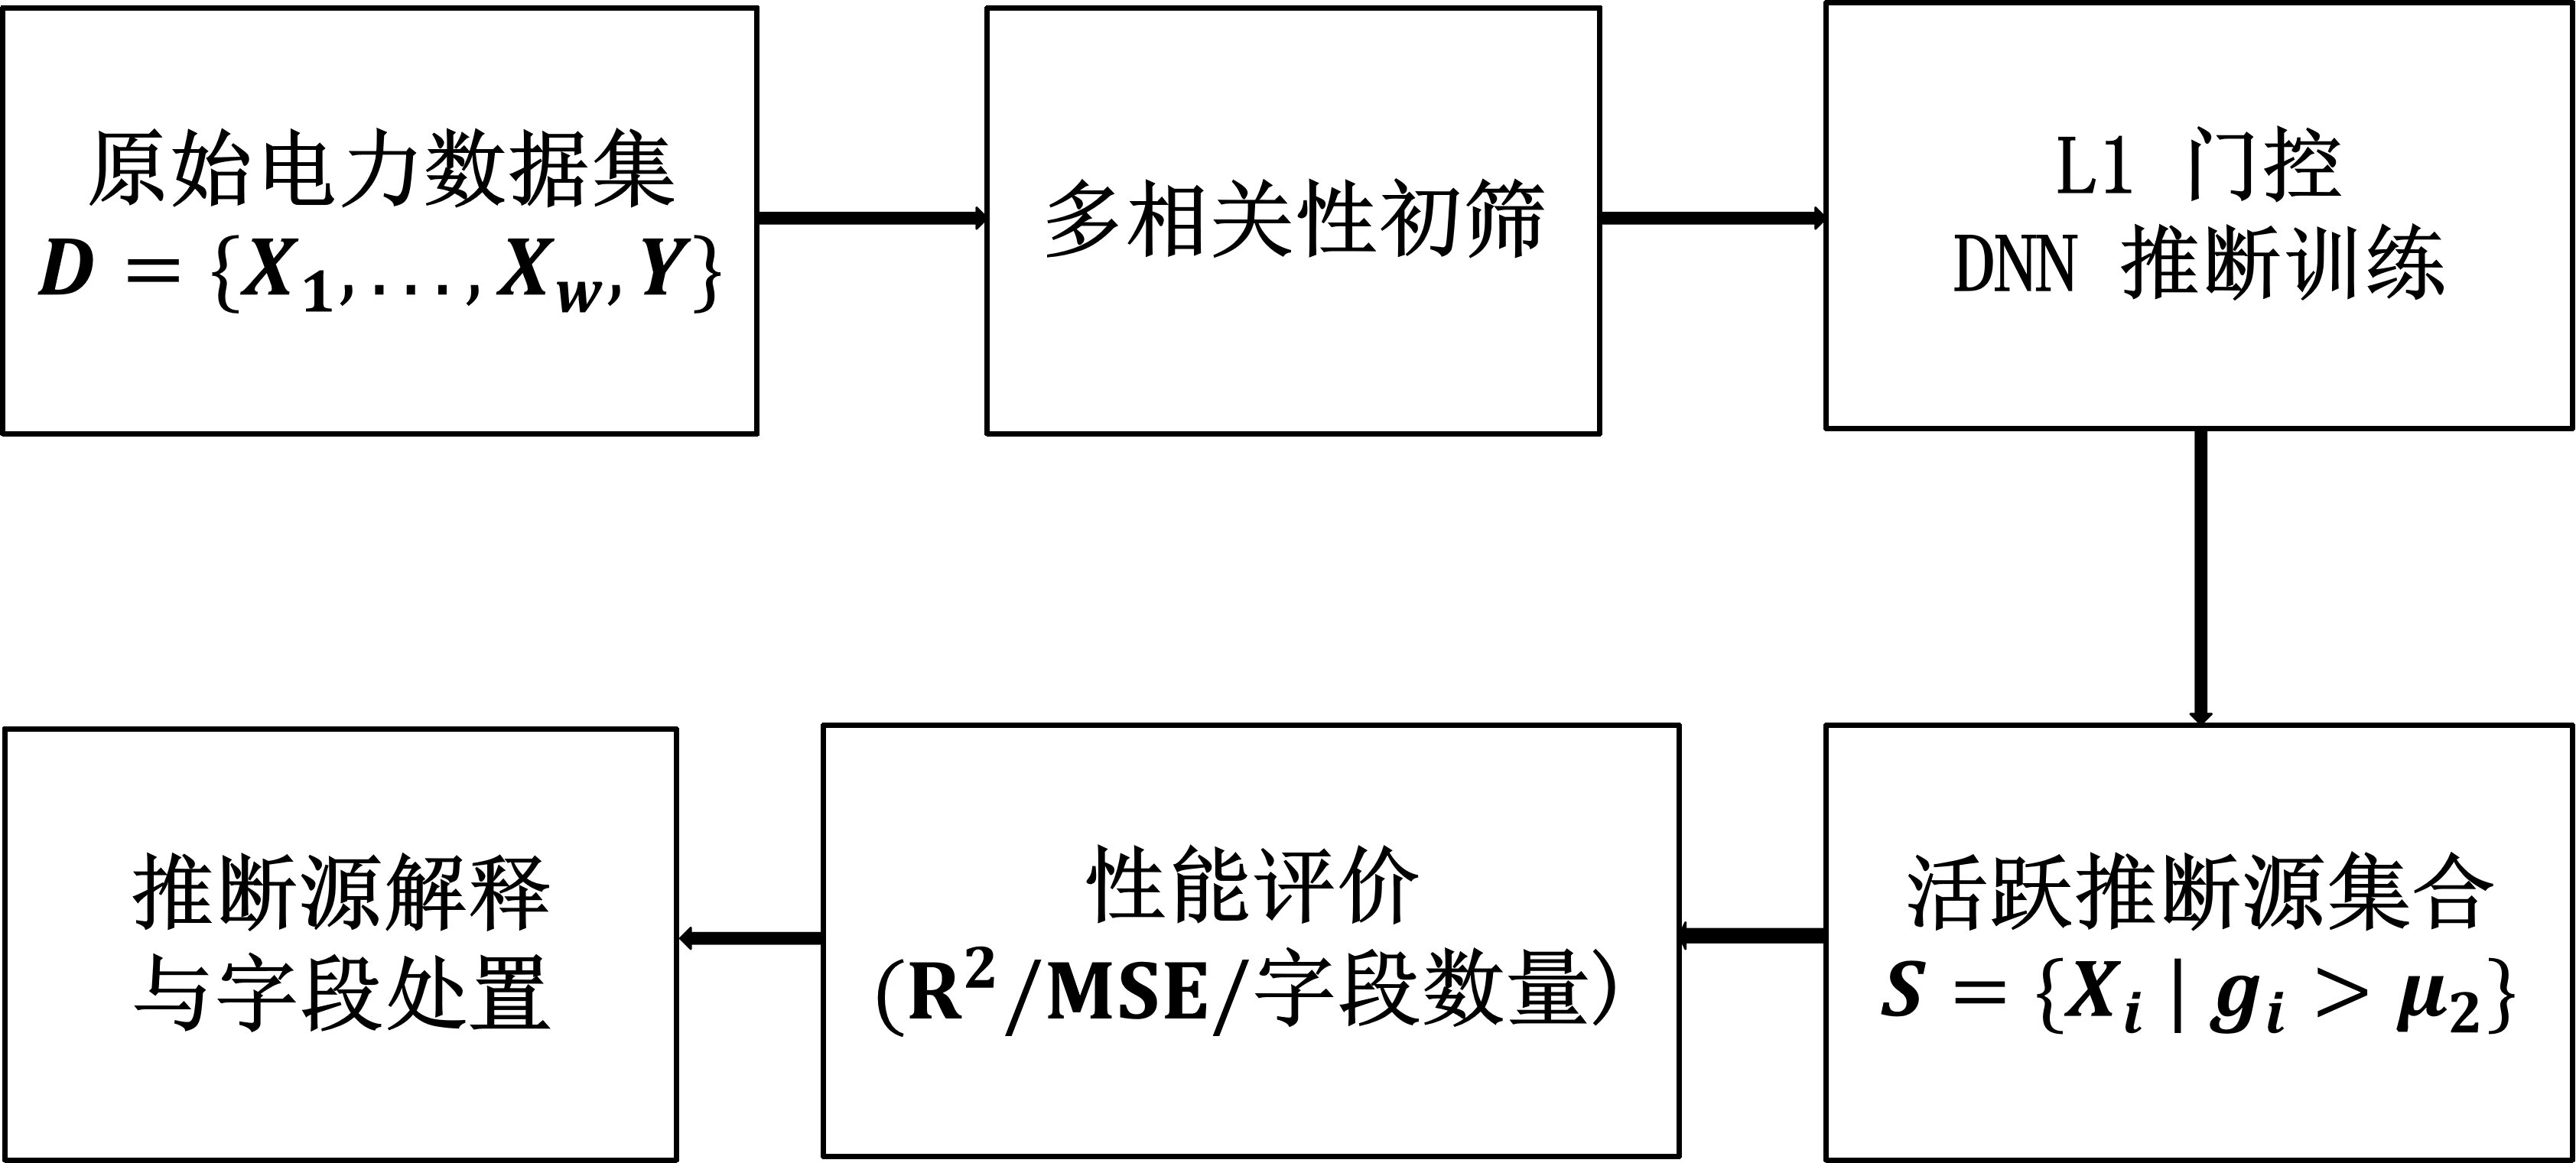
\includegraphics[width=\columnwidth]{总体流程.png}
\figbicaption{隐性推断源定位总体流程}{Overall workflow of implicit inference source localization}
\label{fig:method_flow}
\end{figure}

\subsection{多相关性初筛}
相关系数是刻画变量间关联关系的常用统计工具，其基本思想是将两个变量之间的同步变化程度、排序一致性、分布依赖或核空间依赖压缩为一个可比较的数值\cite{ref-pearson,ref-spearman,ref-kendall}。对于高维电力数据的关联分析而言，相关系数具有两个优点：一是计算效率高，可在大量字段上快速执行；二是结果具有较好的可解释性，便于对候选字段进行初步排序和筛查。但是，相关系数本质上属于描述性统计量，只能说明变量之间存在某种关联，不能直接证明某个字段在联合推断模型中不可替代。因此，本文将相关性分析定位为候选空间压缩和推断线索发现，而不是最终的推断源判定。

电力数据字段之间的依赖关系具有多样性：既可能因潮流方程、功率平衡或数据聚合形成近似线性关系，也可能因市场出清机制、辅助服务约束和分段调度规则产生复杂的非线性耦合。为降低单一统计指标造成的漏筛，本文构建六维相关性向量对每个候选字段 $X_i$ 进行综合评估：
\begin{equation}
R_i=[r_i^{(\metric{NMI})},r_i^{(\metric{Spear})},r_i^{(\metric{Pear})},
r_i^{(\metric{Ken})},r_i^{(\metric{DC})},r_i^{(\metric{HSIC})}].
\end{equation}
式中：六个分量分别对应归一化互信息（NMI）、Spearman 秩相关系数、Pearson 相关系数、Kendall 秩相关系数、距离相关系数（DC）和 Hilbert-Schmidt 独立性准则（HSIC）。六类指标的作用侧重点不同。

Pearson 相关系数度量两个变量之间的线性相关程度，其定义为
\begin{equation}
\rho_{p}(X_i,Y)=
\frac{\mathrm{cov}(X_i,Y)}{\sigma_{X_i}\sigma_Y}.
\end{equation}
当字段之间存在近似线性派生关系或同步波动时，Pearson 系数能够给出直接反映。Spearman 相关系数先将变量转换为秩序列，再计算秩序列的 Pearson 相关，适合刻画单调但非严格线性的关系。Kendall 秩相关系数基于样本对的一致序和逆序关系定义，能够从排序一致性的角度反映变量间关联，对异常值和局部非线性变化相对稳健。

归一化互信息从信息论角度度量变量之间共享信息量，能够发现非单调和非线性依赖\cite{ref-cover-info}。本文将互信息按变量熵进行归一化，使其落入可比较范围。距离相关系数基于样本间距离矩阵度量变量依赖，当且仅当变量独立时其理论值为 0，因而能够捕捉一般形式的非线性关系\cite{ref-szekely-dcorr}。HSIC 则将变量映射到再生核 Hilbert 空间中，通过核矩阵的相关性度量统计依赖，适合刻画复杂非线性耦合\cite{ref-gretton-hsic}。本文同时采用上述六类指标，是因为电力数据中线性、单调、非单调和高阶非线性依赖往往并存，任何单一指标都难以覆盖全部潜在推断路径。

初筛流程如图~\ref{fig:screening_flow} 所示。对每个候选字段，先分别计算六类相关性得分，并将不同指标的得分与对应阈值比较；随后采用“任一指标通过即保留”的宽松策略，即当任意一个指标达到预设阈值时，该字段即被保留进入后续门控建模：
\begin{equation}
\max_j I\left(r_i^{(j)}\geq \mu_1^{(j)}\right)>0.
\end{equation}
式中：$I(\cdot)$ 为示性函数；$\mu_1^{(j)}$ 为第 $j$ 类指标的初筛阈值。该策略的设计原则是宁可保留部分弱冗余字段，也不在早期排除可能具有互补推断作用的字段。换言之，初筛阶段强调召回率和候选覆盖，而不追求最终字段集合的最小化。字段是否真正构成隐性推断源，需要在后续 L1 门控模型中由推断误差和稀疏约束共同决定。

\begin{figure}[!tbp]
\centering
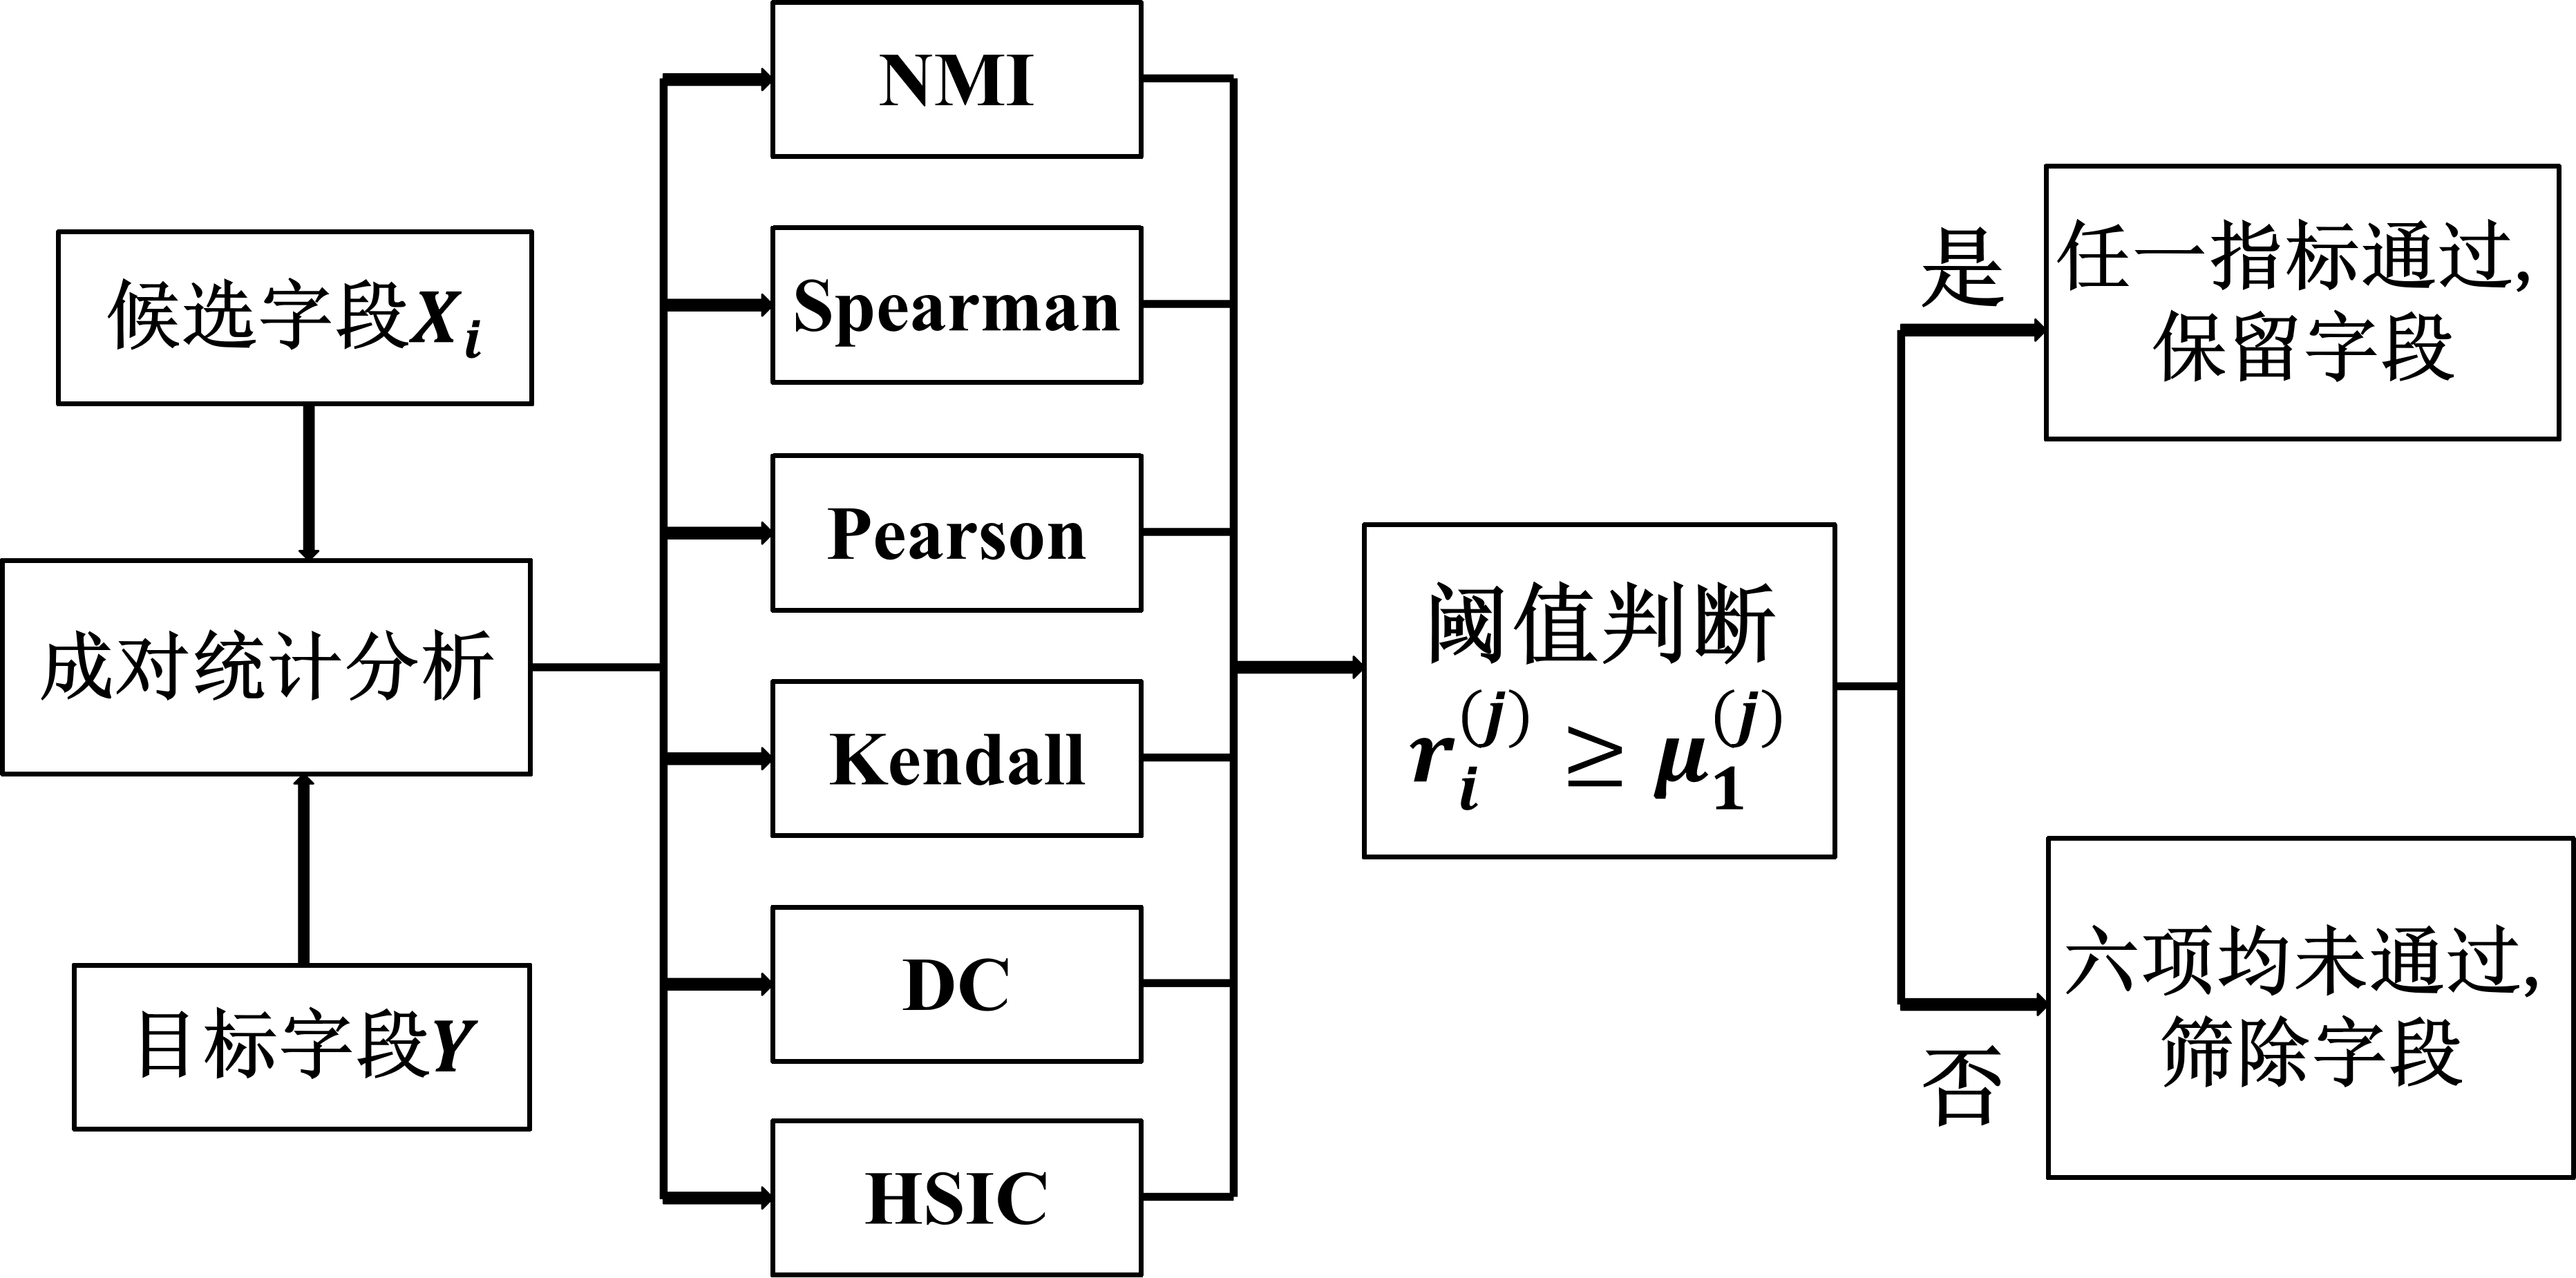
\includegraphics[width=\columnwidth]{初筛流程.png}
\figbicaption{多相关性初筛流程}{Multi-correlation preliminary screening workflow}
\label{fig:screening_flow}
\end{figure}

\subsection{L1 门控深度推断模型}
经过多相关性初筛后，得到候选字段集合 $X=\{X_1,\ldots,X_m\}$，其中 $m$ 为通过初筛的字段数。相关性初筛能够删除明显弱相关字段，但仍会保留大量在统计上有关联、在推断模型中却可能相互替代的字段。若直接使用全部初筛字段训练普通 DNN，模型虽然可能取得较高 $R^2$，但无法说明哪些输入字段承担主要推断作用。为此，本文在深度神经网络的输入端引入可学习门控层，其结构如图~\ref{fig:l1_structure} 所示。

\begin{figure}[!tbp]
\centering
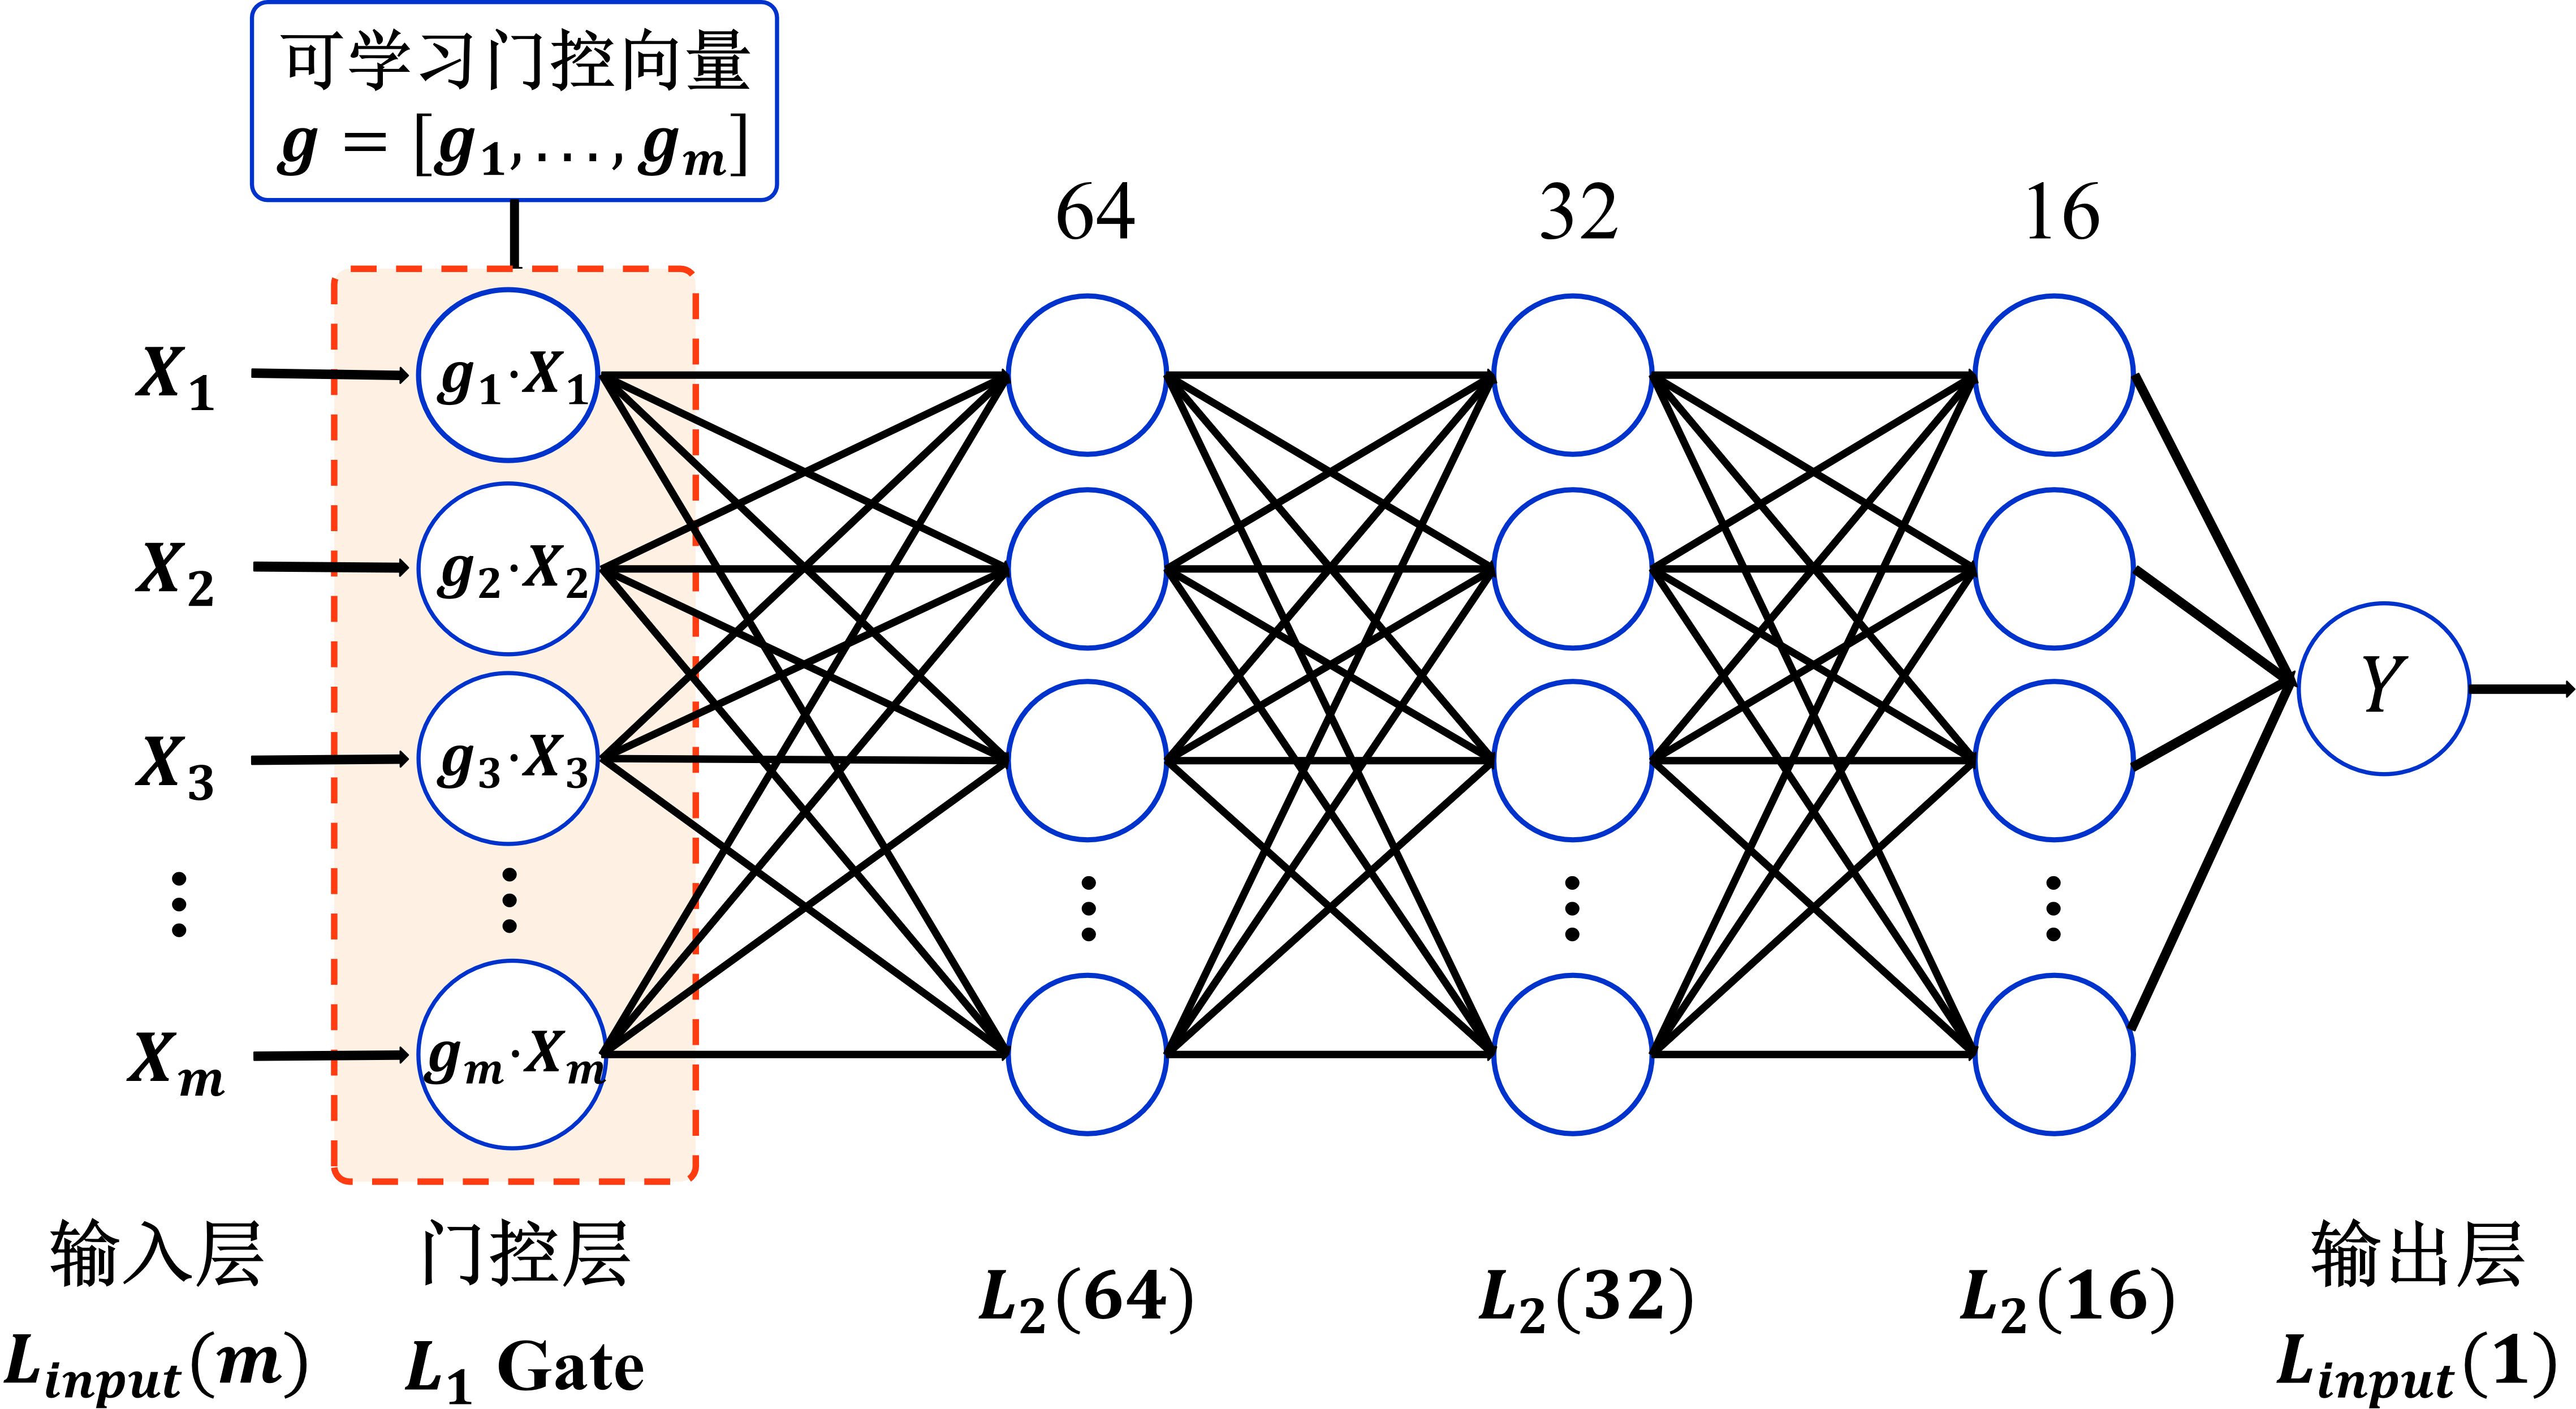
\includegraphics[width=\columnwidth]{门控.png}
\figbicaption{L1 门控深度推断模型结构}{Structure of the L1-gated deep inference model}
\label{fig:l1_structure}
\end{figure}

设门控向量为 $g=[g_1,\ldots,g_m]$，其中 $g_i$ 与候选字段 $X_i$ 一一对应。门控层对输入字段进行逐元素加权，模型输出为
\begin{equation}
\hat{Y}=f_{\theta}(g\odot X),
\end{equation}
式中：$\odot$ 为逐元素相乘运算；$f_{\theta}$ 为由多层全连接网络构成的非线性推断模型。当 $g_i$ 较大时，字段 $X_i$ 的信息能够较充分地进入后续网络；当 $g_i$ 接近 0 时，该字段在前向传播中被显著抑制。为了使门控值既服务于推断精度，又能够产生稀疏选择结果，训练目标函数定义为
\begin{equation}
\mathcal{L}=\frac{1}{n}\sum_{k=1}^{n}(y_k-\hat{y}_k)^2+\lambda\sum_{i=1}^{m}|g_i|.
\end{equation}
式中：第一项为均方误差损失，用于保证模型对目标字段的推断能力；第二项为 L1 正则化惩罚，$\lambda$ 为正则化系数，用于推动门控参数趋向稀疏。该目标函数体现了字段选择中的竞争机制：若某字段能够稳定降低预测误差，反向传播会保留或增大其门控值；若某字段主要提供重复信息、弱相关扰动或噪声，L1 惩罚会持续压低其门控值。与先训练模型再事后解释特征重要性不同，L1 门控将字段筛选嵌入推断模型训练过程，使字段取舍直接受到目标推断误差约束。

训练结束后，满足
\begin{equation}
|g_i|\geq \mu_2
\end{equation}
的字段被判定为活跃推断源。式中 $\mu_2$ 为活跃阈值。本文将活跃字段数量记为 $n_s$，并在后续基线对比实验中作为统一字段预算，使不同方法在相同字段数量约束下进行公平比较。为检验门控筛选结果是否独立有效，本文不直接把门控模型的训练结果作为最终结论，而是将选中字段重新输入普通 DNN 进行训练和测试。若再训练模型仍能保持较高 $R^2$，则说明该字段集合确实包含支撑目标字段推断的主要信息。

\subsection{相关性驱动的改进门控}
普通 L1 门控模型能够在推断训练过程中识别活跃字段，但每个门控参数都是独立学习的变量，尚不能直接回答“六种相关性指标分别对最终推断源判定贡献多少”这一问题。前述六类相关性指标虽然提供了统计依赖证据，但在普通流程中主要用于初筛，其作用仍停留在描述性分析层面，没有与最终推断导向的门控判定形成统一融合机制。换言之，初筛阈值能够决定某个字段是否进入候选空间，却不能解释不同相关性指标如何共同影响门控打开或关闭。

另外考虑一种实际情况：假设数据共享方新增一列候选字段，若仍采用普通 L1 门控方法，通常需要把新字段并入候选集合并重新训练推断模型，才能判断其是否构成推断源。若能够学习出不同相关性指标对推断贡献的权重，则可先计算新字段与目标字段之间的六维相关性向量，再通过统一映射快速得到其推断贡献度，从而降低增量字段分析的计算成本。基于这一考虑，本文进一步提出相关性驱动的改进门控模型，其结构如图~\ref{fig:improved_gate_structure} 所示。

\begin{figure}[!tbp]
\centering

\includegraphics[width=\columnwidth]{改进门控.png}
\figbicaption{相关性驱动的改进门控层结构}{Structure of the correlation-driven improved gate layer}
\label{fig:improved_gate_structure}
\end{figure}

改进门控不再为每个字段直接设置相互独立的自由门控参数，而是将字段 $X_i$ 的六维相关性向量 $R_i$ 作为门控生成依据，通过线性映射和 Sigmoid 激活函数得到门控值：
\begin{equation}
g_i=\sigma(W^{\mathrm{T}}R_i+b),
\end{equation}
式中：$W\in\mathbb{R}^{6}$ 为六类相关性指标对应的可学习权重向量，反映各指标对推断源判定的相对贡献；$b$ 为全局偏置项，可理解为整体的门控开启容忍水平；$\sigma(\cdot)$ 为 Sigmoid 激活函数：
\begin{equation}
\sigma(z)=\frac{1}{1+\mathrm{e}^{-z}}.
\end{equation}
Sigmoid 函数将任意实数映射到 $(0,1)$ 区间，使门控值可以解释为字段被打开的连续强度。当 $z$ 较大时，$\sigma(z)$ 接近 1，字段信息被保留；当 $z$ 较小时，$\sigma(z)$ 接近 0，字段信息被抑制。更重要的是，Sigmoid 在 $z=0$ 处的输出恰好为 0.5，因此当 $W^{\mathrm{T}}R_i+b=0$ 时，$g_i=0.5$。这一性质使 0.5 不再是经验指定的阈值，而是由门控函数形式自然给出的开闭分界点，对应如下判定函数：
\begin{equation}
W^{\mathrm{T}}R_i+b=0.
\end{equation}
Sigmoid 的导数为 $\sigma'(z)=\sigma(z)(1-\sigma(z))$，在 $z=0$ 处取得最大值 0.25。这意味着当综合得分 $W^{\mathrm{T}}R_i+b$ 位于临界区间附近时，较小的相关性证据差异会引起较明显的门控变化；而当得分远离临界区间时，门控趋近饱和，字段保留或抑制状态相对稳定。当 $g_i>0.5$ 时，说明字段 $X_i$ 的综合相关性证据足以支持门控打开，该字段更可能作为潜在推断源进入模型；当 $g_i<0.5$ 时，说明其综合证据不足，该字段更可能为冗余或低贡献字段。训练过程中，$W$、$b$ 与 DNN 主干参数共同优化，并受到推断误差和门控稀疏约束的共同影响。因此，$W$ 的大小不仅反映某类相关性指标的统计强弱，还反映该指标在当前目标推断任务中的有效贡献。

与普通 L1 门控相比，改进门控的主要价值并不在于单纯追求更高的 $R^2$，而在于把“多种相关性证据如何共同影响字段推断源判定”转化为可学习的门控评分函数。对于已有字段，模型能够解释不同相关性指标对门控开闭的贡献；对于新进入的数据字段，若其与目标字段之间的六维相关性已知，则可通过 $g_i=\sigma(W^{\mathrm{T}}R_i+b)$ 快速计算其推断贡献度，在不立即重训完整推断模型的情况下获得初步判定。这种设计使相关性分析从独立初筛工具进一步转化为推断导向的快速评估机制。

\section{实验与结果分析}
\subsection{实验设置}
\subsubsection{数据集}
实验采用美国 PJM 互联电网 2025 年小时级市场与运行公开数据\cite{ref-pjm-dataminer}。该数据涵盖能量市场、辅助服务、负荷、发电结构和交换功率等多个业务环节，字段之间同时受到电力系统物理规律与市场运行机制的影响，具有多源、异构和关联关系复杂等特点，适合用于验证所提方法对电力数据推断源的识别能力。


该数据集包含 8760 行（对应全年逐小时记录）和 72 列，其中前两列为 UTC 和东部时间的时间戳，仅用于时间对齐，不参与建模分析。去除时间字段后，剩余 70 个数据字段可按照 PJM Data Miner 官方数据源定义划分为如表~\ref{tab:data_overview} 所示的类别。数据涵盖发电与损耗、风电光伏出力、燃料类型发电、负荷预测与计量、调频市场、辅助服务市场、节点电价和交换功率等多个业务领域，字段间存在广泛的物理和市场机制关联。

\begin{table}[!tbp]
\centering
\scriptsize
\setlength{\tabcolsep}{2pt}
\tabbicaption{PJM 2025 数据字段分类概览}{Classification of PJM 2025 data fields}
\label{tab:data_overview}
\begin{tabularx}{\columnwidth}{c>{\raggedright\arraybackslash}p{0.40\columnwidth}X}
\toprule
编号 & Dataset & 中文说明 \\
\midrule
D1--D2 & Generation and EHV Losses & 小时级总发电量与超高压损耗数据。 \\
D3 & Wind Generation & PJM 区域小时级风电出力。 \\
D4 & Solar Generation & PJM 区域小时级光伏出力。 \\
D5--D24 & Generation by Fuel Type & 按燃料类型统计的发电出力与占比。 \\
D25--D26 & Historical Load Forecasts & 日前及最新可用负荷预测。 \\
D27 & Hourly Load: Preliminary & 由遥测数据计算的预估小时负荷。 \\
D28 & Hourly Load: Metered & PJM RTO 服务区域计量负荷。 \\
D29--D37 & Regulation Billing Data & 调频市场预结算相关价格、容量与信用数据。 \\
D38--D56 & Day-Ahead AS Market Results & 日前辅助服务市场的价格、需求与容量结果。 \\
D57--D60 & Day-Ahead Hourly LMPs & 日前能量市场 LMP、拥塞价与边际损耗价。 \\
D61--D64 & Real-Time Hourly LMPs & 实时能量市场 LMP、拥塞价与边际损耗价。 \\
D65--D70 & Actual/Schedule Summary & 净/总实际、计划和非计划交换功率。 \\
\bottomrule
\end{tabularx}
\end{table}

\subsubsection{参数设置}
多相关性初筛阶段的各项阈值设置如下：归一化互信息（NMI）为 0.06、Spearman 秩相关系数为 0.15、Pearson 相关系数为 0.15、Kendall 秩相关系数为 0.12、距离相关系数为 0.20、HSIC 为 0.25。上述阈值均用于"任一指标通过即保留"的宽松初筛规则。深度神经网络主干结构采用三层全连接隐藏层，各层神经元数量依次为 64、32 和 16；优化器采用 Adam\cite{ref-kingma-adam}；批次大小设为 50；训练轮数为 200；随机种子固定为 42 以保证实验可重复性。普通 L1 门控模型的 L1 正则化系数 $\lambda$ 设为 0.002，活跃阈值 $\mu_2$ 设为 0.10。改进 L1 门控模型的门控判定阈值为 0.50，L1 正则化系数设为 0.016，权重向量 $W$ 和偏置 $b$ 分别配置独立学习率，以确保相关性权重和门控偏置的稳定收敛。

\subsubsection{实验设计}
围绕方法执行过程、基线方法对比和冗余输入影响本文设计了三组实验，分别对应第 3.2--3.4 节。

第一组为单目标下全量模型与 L1 门控模型的直接对比，以净实际交换功率为目标字段。全量 DNN 使用除当前目标外的 69 个字段进行训练，L1DNN 则先由 L1 门控模型获取活跃字段集合，再以相同的 DNN 结构重新训练并评估推断性能。该组实验旨在完整展示L1DNN在单一目标上的执行过程与结果分析，并验证净实际交换功率在字段压缩后是否仍能保持甚至提升推断能力。

第二组为同预算基线对比。参与对比的方法包括 NMI、Pearson、Spearman 排序选择，Lasso、ElasticNet，以及随机森林和 XGBoost 特征重要性排序。对于每个目标字段，各方法分别按照自身的排序结果选取 Top-$k$ 字段，并统一采用普通 DNN 进行训练和测试，其中字段数 $k$ 从小到大递增。当任意一种方法的测试 $R^2$ 首次达到全量 DNN 的 95\%（或 97\%）水平时，即将对应字段数确定为该目标下所有方法的统一预算 $n$。随后比较各方法在相同字段数 $n$ 下的测试结果，从而消除字段数量差异的影响，使对比聚焦于不同方法的字段选择质量。

第三组为冗余输入影响分析。针对日前拥塞价和主备用容量这两个在字段压缩后测试精度反而明显上升的代表性目标，比较全量字段、L1 选中字段和不同 Top-n 字段的训练曲线与测试 $R^2$，分析少量字段推断精度优于全量字段的内在原因，揭示冗余和弱相关字段对模型泛化性能的影响机制。

\subsection{单目标推断源识别与门控演化}
净实际交换功率是反映区域电网与外部系统功率交换状态的核心运行量，其变化同时受负荷水平、发电结构、备用需求和市场出清结果影响，具有较高的数据价值和较复杂的关联来源。为展示所提方法的完整执行过程，首先以该字段为单一目标，分析多相关性初筛、L1 门控收缩、Top-n 再训练验证以及改进门控权重学习结果。

\subsubsection{多相关性初筛结果}
以净实际交换功率为中心目标，共有 69 个候选关系参与初筛分析。经六类指标综合评估后，保留 55 个候选字段，筛除 14 个与目标明显弱相关的字段。各类指标的通过数量分别为：NMI 23 个、Spearman 33 个、Pearson 25 个、Kendall 29 个、距离相关系数 27 个、HSIC 31 个。各字段通过指标数的分布情况为：0 项（即被筛除）14 个、1 项 19 个、2 项 5 个、3 项 5 个、4 项 10 个、5 项 12 个、6 项（全部通过）4 个。

表~\ref{tab:screening_top} 按最大绝对相关得分从高到低给出初筛结果的节选。可以观察到，辅助服务市场字段、交换功率相关字段和燃料结构字段在多类指标下均表现出较强的统计依赖性，表明净实际交换功率的潜在推断路径涉及多个业务领域，并非由单一线性相关关系所决定。

\begin{table}[!tbp]
\centering
\scriptsize
\setlength{\tabcolsep}{1pt}
\tabbicaption{净实际交换功率目标的多相关性初筛结果节选}{Partial multi-correlation screening results for net actual interchange}
\label{tab:screening_top}
\begin{tabularx}{\columnwidth}{cXrrrrrrc}
\toprule
排名 & 字段 & NMI & Spear. & Pear. & Kend. & DC & HSIC & 通过数 \\
\midrule
1 & 30 min备用实际量 & 0.076 & -0.430 & -0.394 & -0.289 & 0.403 & 0.856 & 6 \\
2 & 30 min备用总量 & 0.067 & -0.428 & -0.397 & -0.252 & 0.374 & 0.845 & 6 \\
3 & 总计划交换功率 & 0.133 & -0.465 & -0.483 & -0.318 & 0.458 & 0.813 & 6 \\
4 & 核电出力 & 0.116 & -0.354 & -0.424 & -0.248 & 0.442 & 0.795 & 6 \\
\multicolumn{9}{c}{\(\cdots\)} \\
53 & 实时拥塞价 & 0.013 & 0.124 & 0.155 & 0.091 & 0.182 & 0.032 & 1 \\
54 & 同步备用MCP & 0.050 & 0.175 & 0.133 & 0.111 & 0.134 & 0.063 & 1 \\
55 & 日前拥塞价 & 0.073 & -0.039 & -0.066 & -0.048 & 0.171 & 0.070 & 1 \\
\bottomrule
\end{tabularx}
\end{table}

\subsubsection{推断精度与门控收缩过程}
图~\ref{fig:train_pair} 对比展示了净实际交换功率目标上全量 DNN 和 L1 门控模型的训练过程。全量 DNN 以 69 个候选字段训练，最优测试 $R^2$ 为 0.9675；L1 门控模型在初筛后的 55 个字段上训练，最优测试 $R^2$ 达到 0.9775。结果表明，稀疏门控约束不仅未削弱模型推断能力，反而在当前数据划分下提升了泛化性能。其原因在于，L1 门控在训练过程中持续压缩冗余字段的贡献，迫使模型更集中地利用稳定的推断路径，从而降低了过拟合倾向。

\begin{figure}[!tbp]
\centering
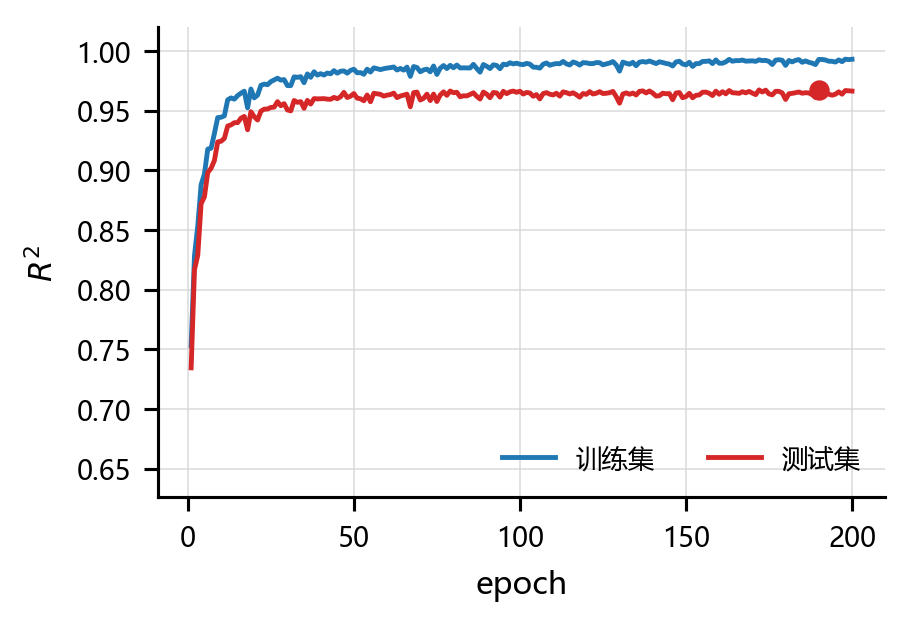
\includegraphics[width=\columnwidth]{net_train_dnn_r2_zh.png}\\[-0.2em]
{\scriptsize (a) 全量 DNN}\\[0.45em]
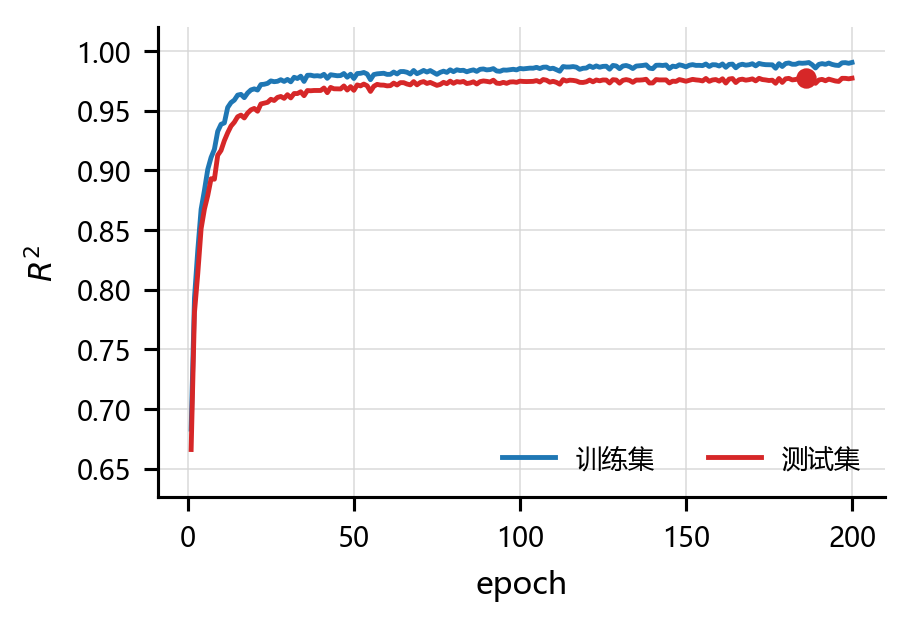
\includegraphics[width=\columnwidth]{net_train_l1_r2_zh.png}\\[-0.2em]
{\scriptsize (b) L1 门控模型}
\figbicaption{净实际交换功率目标上的 $R^2$ 训练过程对比}{Comparison of training $R^2$ processes for net actual interchange}
\label{fig:train_pair}
\end{figure}

图~\ref{fig:l1_gate} 展示了 L1 门控模型的门控参数演化过程，图中每条曲线对应一个候选字段的门控值随训练轮次的变化轨迹。在训练初期，各字段的门控值即出现明显分化；随着 L1 正则化惩罚的持续作用，大量弱贡献字段的门控值逐步衰减至阈值以下，仅有少数关键字段维持较高的门控值。在活跃阈值 $\mu_2=0.10$ 下，最终保留 18 个活跃字段，其中包含天然气发电出力、煤电出力、实时负荷、计量负荷、预估小时负荷和光伏发电出力等关键运行变量；表~\ref{tab:l1_gate_values} 给出了最终门控值排名靠前的部分字段。图~\ref{fig:l1_active} 进一步展示了活跃字段数量随训练轮次的变化趋势，可以观察到活跃字段数量呈现逐步下降并趋于稳定的特征。这说明 L1 门控并非在训练结束时一次性截断弱字段，而是在优化过程中通过梯度信息逐步识别并剔除冗余字段，最终形成紧凑的推断源集合。

\begin{table}[!tbp]
\centering
\scriptsize
\setlength{\tabcolsep}{3pt}
\tabbicaption{净实际交换功率目标的部分最终门控参数值}{Partial final gate values for net actual interchange}
\label{tab:l1_gate_values}
\begin{tabularx}{\columnwidth}{cXc}
\toprule
排序 & 字段 & 最终门控值 \\
\midrule
1 & 天然气发电出力 & 0.894 \\
2 & 实时负荷 & 0.774 \\
3 & 煤电出力 & 0.751 \\
4 & 预估小时负荷 & 0.723 \\
5 & 计量负荷 & 0.614 \\
6 & 光伏发电出力 & 0.552 \\
7 & 核电出力 & 0.444 \\
8 & 水电出力 & 0.388 \\
9 & 风电预测出力 & 0.239 \\
10 & 风电燃料类型出力 & 0.185 \\
\bottomrule
\end{tabularx}
\end{table}

\begin{figure}[!tbp]
\centering

\includegraphics[width=\columnwidth]{net_l1_gate_params_zh.png}
\figbicaption{净实际交换功率目标上门控参数的演化过程}{Evolution of gate parameters for net actual interchange}
\label{fig:l1_gate}
\end{figure}

\begin{figure}[!tbp]
\centering

\includegraphics[width=\columnwidth]{net_l1_active_features_zh.png}
\figbicaption{净实际交换功率目标上活跃字段数量的变化}{Number of active features over training epochs}
\label{fig:l1_active}
\end{figure}

\subsubsection{Top-n 推断源验证}
为独立验证 L1 门控所选字段是否具备实际推断能力，本文按最终门控值从大到小排序，依次取 Top3、Top6、Top9、Top12、Top15、Top18 字段，分别训练普通 DNN 并评估其测试 $R^2$，同时与全量 69 字段和未选中 51 字段的结果进行比较。实验结果如图~\ref{fig:top_series} 所示。

当字段数较少时，推断能力受到明显限制：Top3 和 Top6 的测试 $R^2$ 分别仅为 0.4469 和 0.5778。随着字段数增加，推断能力显著提升：Top9 达到 0.9186，Top15 达到 0.9630，Top18 达到 0.9681，略高于全量 69 字段的 0.9661。与之形成对比的是，去除 Top18 后剩余的 51 个未选中字段单独训练仅取得 0.7820 的测试 $R^2$。上述结果表明，L1 门控识别出的字段集合具有两个重要特征：一是所选字段共同构成了支撑目标推断的核心路径，推断能力甚至略优于全量字段；二是未选中字段尽管数量更多，但缺乏关键推断路径，单独推断能力显著下降。这进一步印证了 L1 门控不是简单挑选个别强相关字段，而是识别出能够联合支撑目标推断的非冗余字段组合。

\begin{figure}[!tbp]
\centering

\includegraphics[width=\columnwidth]{net_top_series_r2_zh.png}
\figbicaption{净实际交换功率目标上的 Top-n 推断源验证结果}{Top-n inference-source validation for net actual interchange}
\label{fig:top_series}
\end{figure}

\subsubsection{改进门控的评分函数学习}
图~\ref{fig:improved_gate} 至图~\ref{fig:improved_b} 展示了相关性驱动改进门控模型的训练结果。与普通 L1 门控模型不同，改进门控的门控值由六维相关性向量经 Sigmoid 映射生成，因此判定阈值设为 0.5，具有明确的数学含义：当 $W^{\mathrm{T}}R_i+b=0$ 时，Sigmoid 输出恰好为 0.5，对应判定边界；高于该边界表示相关性证据足以支持字段作为推断源，低于该边界则表示字段更可能为冗余或低贡献字段。

在本次实验中，改进 L1 门控最终保留 17 个活跃字段，最优测试 $R^2$ 为 0.9726。从权重向量 $W$ 的演化过程来看，HSIC 对应的权重在训练收敛后保持最高，表明非线性依赖证据对净实际交换功率目标的推断源判定贡献最为显著；偏置 $b$ 从接近零的初始值逐步下降至约 $-0.70$，反映出模型在 L1 正则化压力下不断收紧门控打开条件。改进门控的核心意义在于：它将“各类统计指标如何共同影响字段推断源判定”这一问题转化为可学习的门控评分函数，取代了传统方法中需要为每个指标独立设置阈值的方式。

\begin{figure}[!tbp]
\centering

\includegraphics[width=\columnwidth]{improved_l1_gate_params_zh.png}
\figbicaption{改进 L1 门控模型的门控值演化}{Gate value evolution of the improved L1-gated model}
\label{fig:improved_gate}
\end{figure}

\begin{figure}[!tbp]
\centering
\begin{minipage}{\columnwidth}
\centering
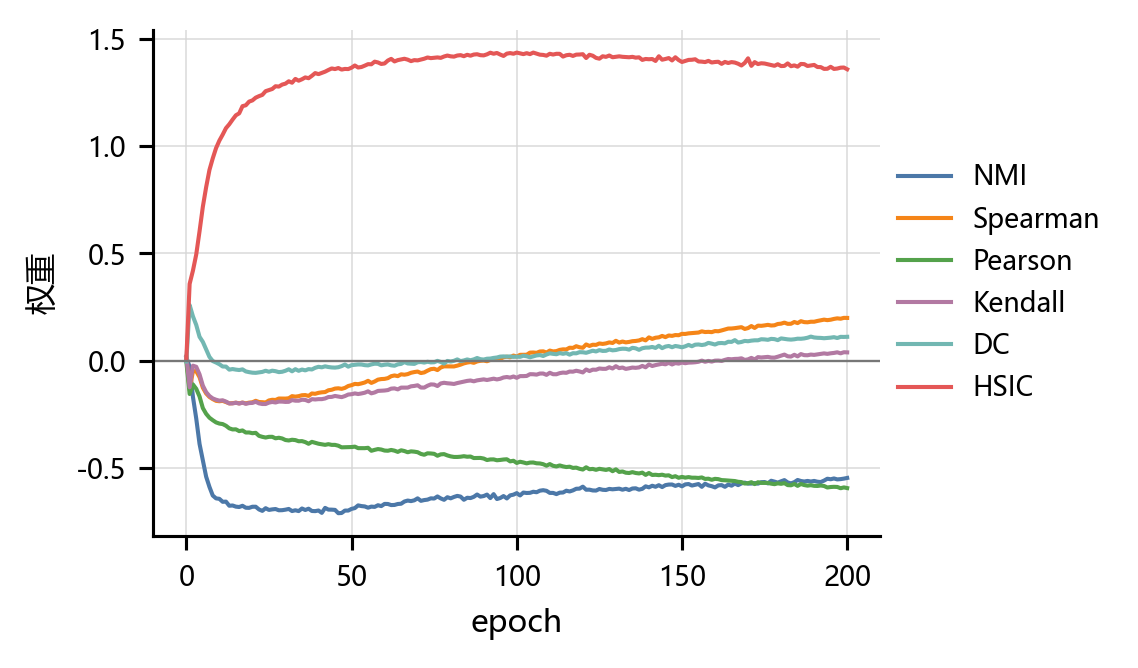
\includegraphics[width=0.92\linewidth]{improved_l1_w_meta_zh.png}\\[-0.4em]
{\scriptsize (a) 相关性指标权重 $W$ 的演化}
\end{minipage}\\[-0.2em]
\begin{minipage}{\columnwidth}
\centering

\includegraphics[width=0.86\linewidth]{improved_l1_b_meta_zh.png}\\[-0.4em]
{\scriptsize (b) 偏置 $b$ 的演化}
\end{minipage}
\figbicaption{改进门控中指标权重与偏置的训练演化}{Evolution of metric weights and bias in the improved gate}
\label{fig:improved_b}
\end{figure}

\subsection{多目标对比实验}
为检验方法在不同类型目标字段上的适用性，本文进一步选取价格、负荷、发电、备用容量和交换功率等 12 个目标开展多目标实验。该组实验关注两个问题：一是 L1 门控在不同业务字段上能否以更少输入维持推断性能；二是在相同字段预算下，门控选择结果是否优于常见相关性排序、线性稀疏模型和树模型重要性排序。

\subsubsection{全量模型与 L1 门控模型对比}
为系统评估所提方法的泛化性能，本文在 12 个目标字段上开展了全量 DNN 与 L1 门控选中特征 DNN 的直接对比实验。全量 DNN 使用除当前目标外的 69 个字段进行训练，L1DNN 则先由 L1 门控模型确定活跃字段集合，再使用相同网络结构重新训练并评估。实验结果如图~\ref{fig:dnn_l1_compare} 和表~\ref{tab:dnn_l1_compare} 所示。

以数据全集中 70 个数值字段扣除目标字段后的 69 个字段作为统一全量基准，全量 DNN 的字段利用率为 100\%，12 个目标的平均测试 $R^2$ 为 0.9031；L1 门控模型平均仅使用 15.50 个字段，字段利用率约为 22.46\%，平均测试 $R^2$ 为 0.9111，高于全量 DNN 的结果。从各目标的具体表现来看，在日前拥塞价、主备用容量、总实际交换功率和净实际交换功率等目标上，L1 门控模型显著或略微优于全量 DNN；在实时拥塞价和日前 LMP 上，L1 门控模型略低于全量 DNN。上述结果表明，所提方法并非对所有目标进行机械式的字段压缩，而是能够在大多数目标上以显著缩减的字段规模保持同等甚至更优的泛化能力。对于少数字段压缩后性能略有下降的目标，其下降幅度有限，仍处于可接受范围。

\begin{figure}[!tbp]
\centering

\includegraphics[width=\columnwidth]{dnn_vs_l1_method_compare_zh.png}
\figbicaption{12 个目标字段上全量 DNN 与 L1 门控模型的测试 $R^2$ 对比}{Comparison of test $R^2$ between all-feature DNN and L1-gated model across 12 targets}
\label{fig:dnn_l1_compare}
\end{figure}

\begin{table}[!tbp]
\centering
\scriptsize
\setlength{\tabcolsep}{2pt}
\tabbicaption{全量 DNN 与 L1 门控选中特征 DNN 的详细对比}{Detailed comparison between all-feature DNN and L1-gated selected-feature DNN}
\label{tab:dnn_l1_compare}
\begin{tabularx}{\columnwidth}{Xrrrr}
\toprule
中心目标 & 全量字段 & L1 字段 & 全量 DNN & L1DNN \\
\midrule
拥塞价 DA & 69 & 2 & 0.9408 & \textbf{0.9954} \\
主备用容量 & 69 & 14 & 0.8495 & \textbf{0.8826} \\
总实际交换 & 69 & 16 & 0.8499 & \textbf{0.8677} \\
30 min 备用容量 & 69 & 22 & 0.8967 & \textbf{0.9086} \\
边际损耗价 DA & 69 & 18 & 0.8936 & 0.8995 \\
净实际交换 & 69 & 18 & 0.9680 & 0.9728 \\
总发电量 & 69 & 16 & 0.9253 & 0.9271 \\
净计划交换 & 69 & 16 & 0.9691 & 0.9694 \\
总损耗 & 69 & 18 & 0.9413 & 0.9409 \\
计量负荷 & 69 & 15 & 0.9157 & 0.9139 \\
日前 LMP & 69 & 13 & \textbf{0.9622} & 0.9510 \\
拥塞价 RT & 69 & 18 & \textbf{0.7255} & 0.7040 \\
\midrule
平均 & -- & 15.5 & 0.9031 & 0.9111 \\
\bottomrule
\end{tabularx}
\end{table}

\subsubsection{同预算基线对比}
同预算基线对比实验的具体做法为：对每个目标按字段数递增搜索，参与对比的各方法独立选取字段并评估，以其中任意一种方法率先使测试 $R^2$ 达到全量 DNN 的 95\% 或 97\% 水平时对应的字段数作为统一预算 $n$ ；随后，所有基线方法在相同字段数 $n$ 下进行字段选择，并统一使用普通 DNN 训练和测试。在此设置下，不同方法的比较聚焦于"在相同字段预算下，谁选择的字段更具推断能力"，而非"谁使用了更多字段"。

图~\ref{fig:budget_lines} 给出了 95\% 和 97\% 统一预算下各目标的测试 $R^2$ 折线对比结果，图~\ref{fig:budget_avg} 进一步汇总了各方法在两种预算下的平均表现。在 95\% 预算水平下，平均字段数为 8.92，L1 门控模型的平均 $R^2$ 为 0.8875，高于随机森林的 0.8562、ElasticNet 的 0.8115、Lasso 的 0.7967 和 XGBoost 的 0.7798；在 97\% 预算水平下，平均字段数增加至 9.75，L1 门控模型的平均 $R^2$ 进一步提升至 0.8943，仍保持最优。在两种预算水平下，单相关性排序方法的整体表现偏低，表明仅依靠 NMI、Pearson 或 Spearman 等单一指标排序难以稳定保留联合推断所需的关键字段；树模型和线性稀疏模型虽在个别目标上具有竞争力，但在平均性能上仍不及 L1 门控模型。上述结果验证了所提方法在统一字段预算约束下的特征选择优势。

\begin{figure}[!tbp]
\centering
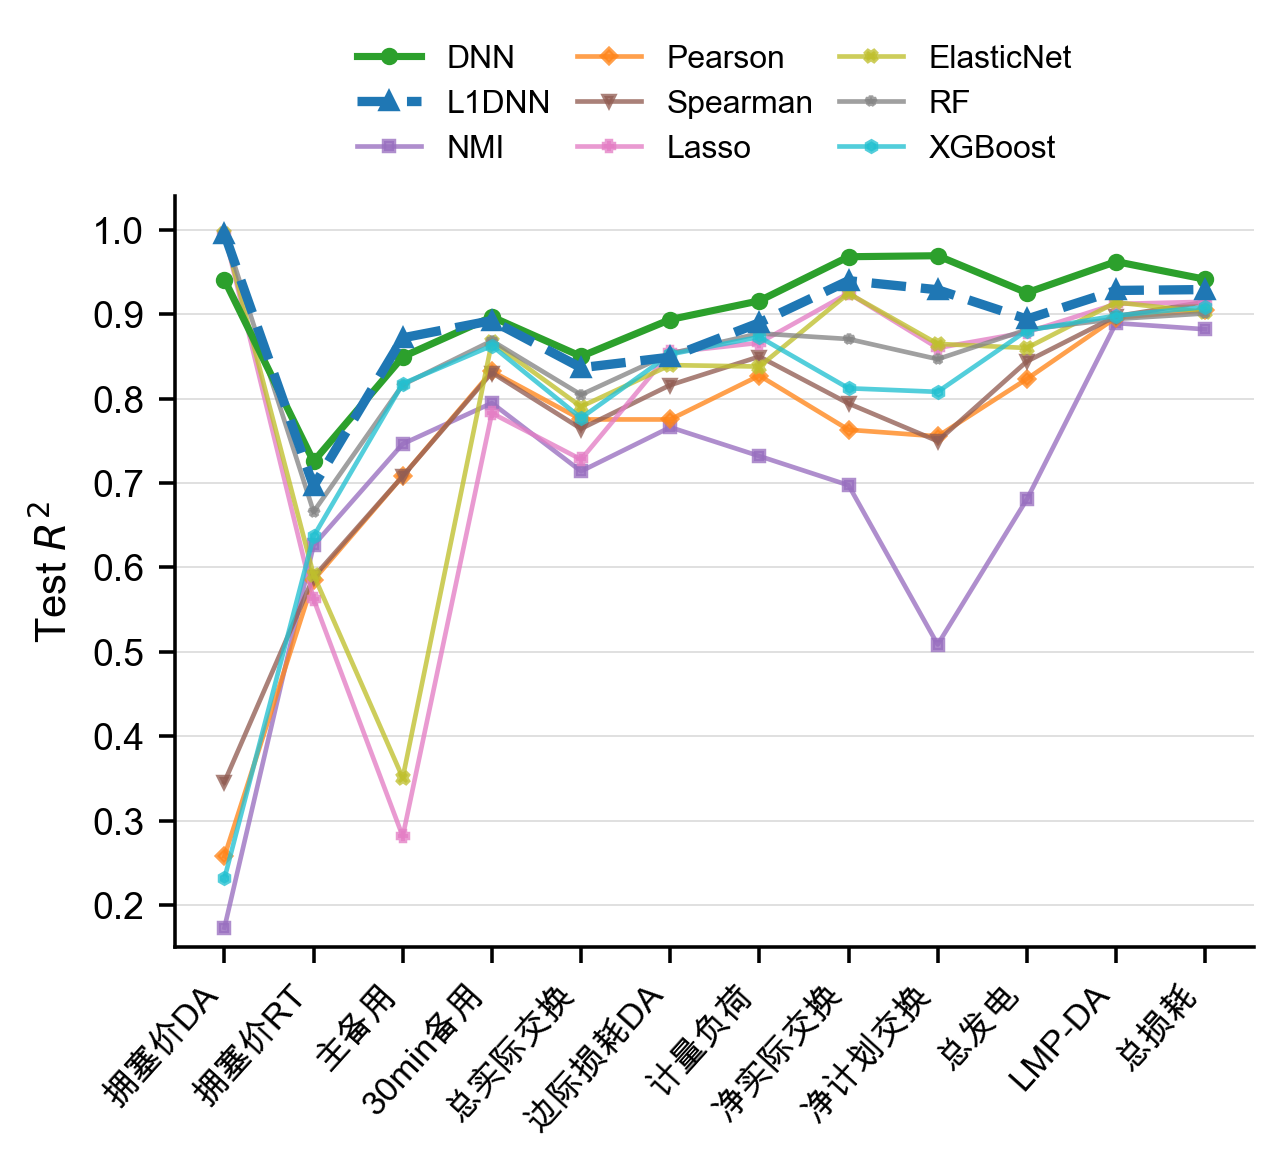
\includegraphics[width=\columnwidth]{budget95_baseline_lines_zh.png}\\[-0.2em]
{\scriptsize (a) 95\% 统一预算}\\[0.45em]
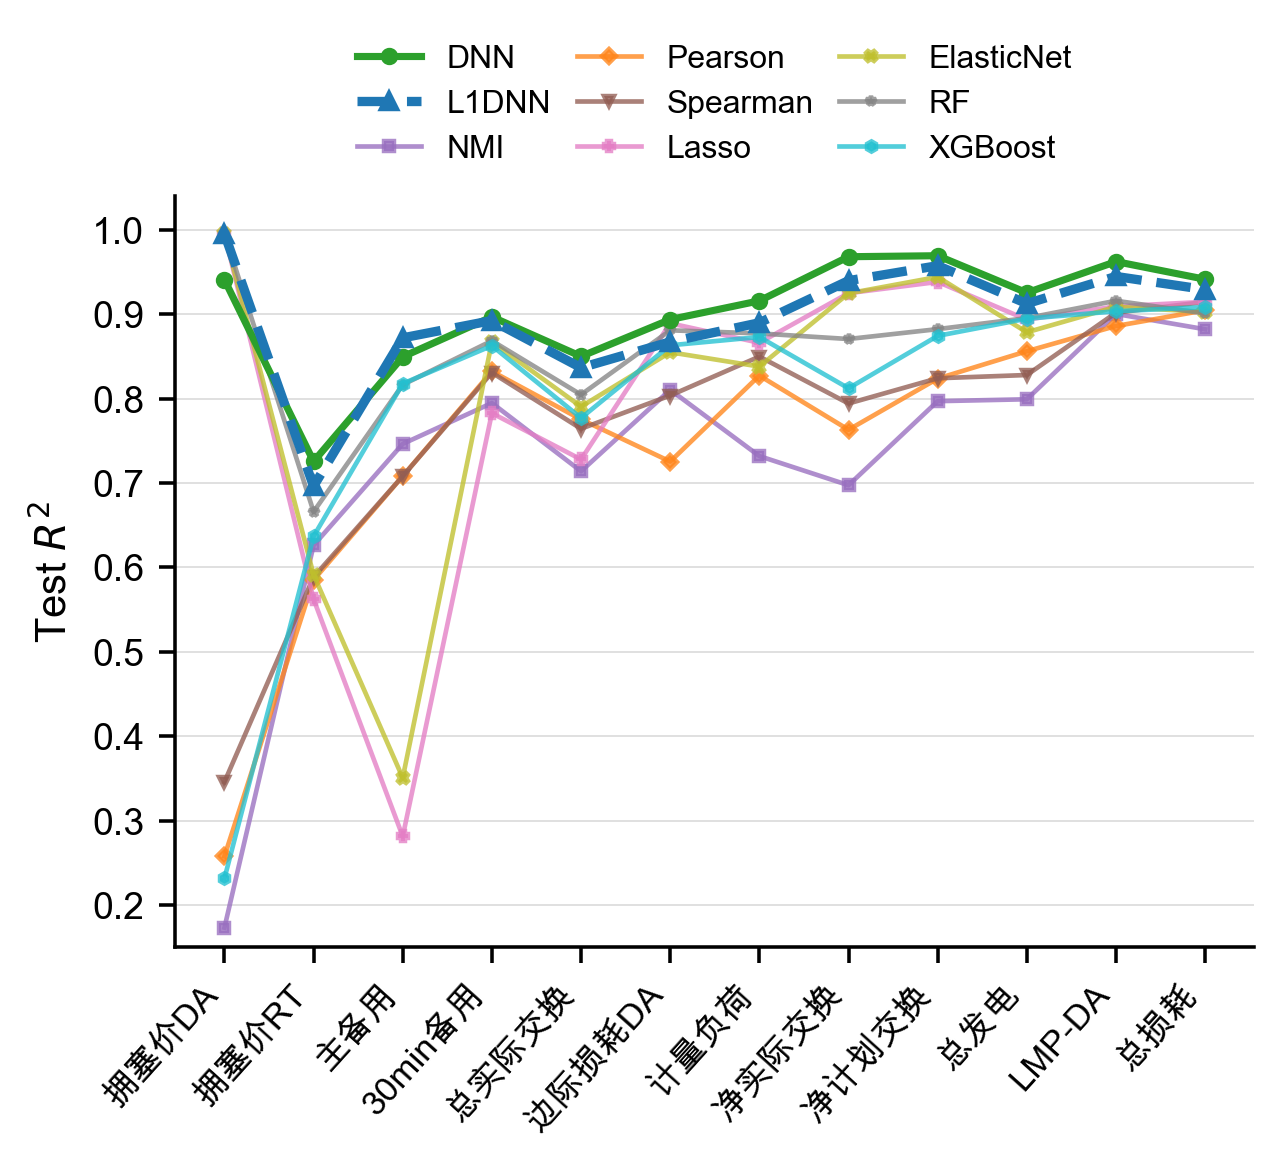
\includegraphics[width=\columnwidth]{budget97_baseline_lines_zh.png}\\[-0.2em]
{\scriptsize (b) 97\% 统一预算}
\figbicaption{统一预算下各目标的基线测试 $R^2$ 对比}{Target-level benchmark comparison under unified feature budgets}
\label{fig:budget_lines}
\end{figure}

\begin{figure}[!tbp]
\centering
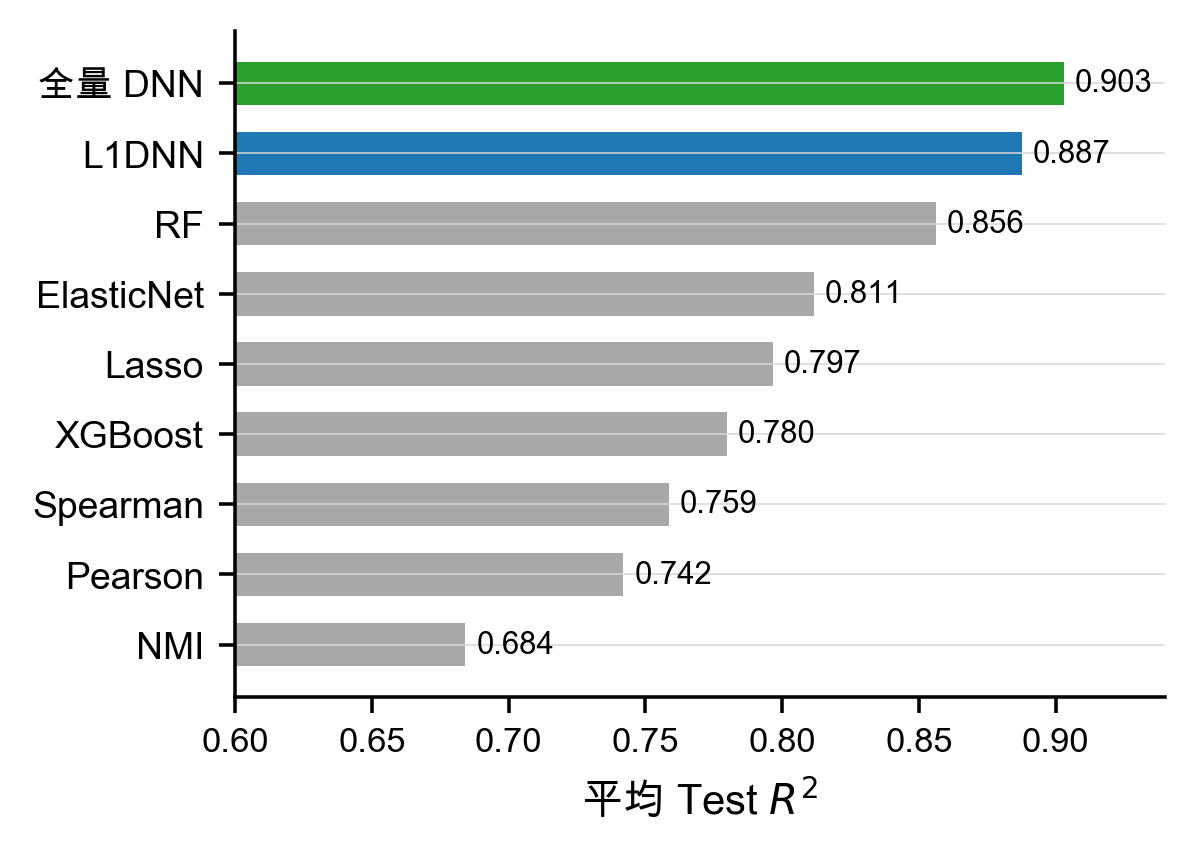
\includegraphics[width=\columnwidth]{budget95_average_bar_zh.png}\\[-0.2em]
{\scriptsize (a) 95\% 统一预算}\\[0.45em]
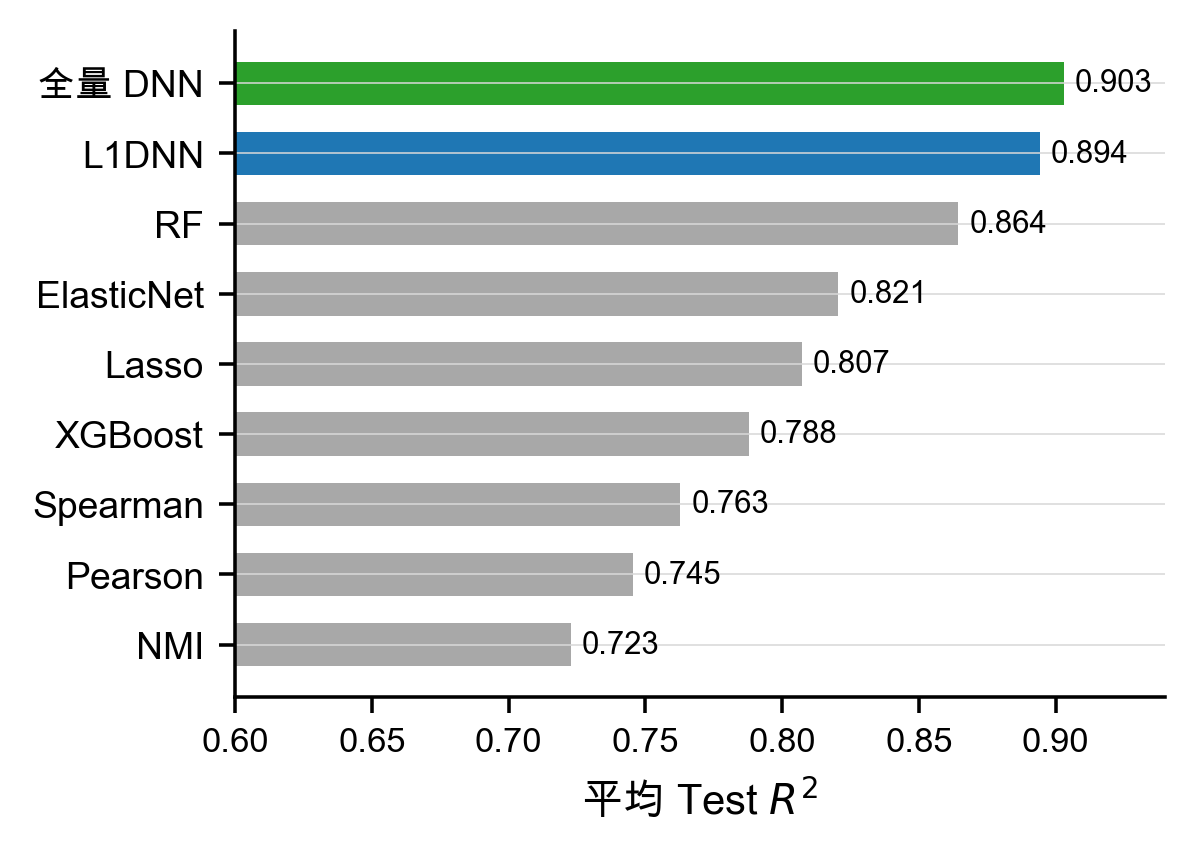
\includegraphics[width=\columnwidth]{budget97_average_bar_zh.png}\\[-0.2em]
{\scriptsize (b) 97\% 统一预算}
\figbicaption{统一预算下各基线方法的平均测试 $R^2$}{Average test $R^2$ of benchmark methods under unified feature budgets}
\label{fig:budget_avg}
\end{figure}

\subsection{冗余输入影响分析}
多目标结果显示，部分目标在压缩字段后测试性能反而高于全量输入。为解释这一现象，本文选取日前拥塞价和主备用容量两个具有代表性的目标，结合训练曲线和 Top-n 递增实验分析冗余字段对模型泛化能力的影响。

\subsubsection{训练曲线对比分析}
在上述实验中，字段压缩后测试性能不降反升这一现象，并不意味着全量字段所含信息量不足，而是揭示出全量输入中冗余和噪声字段对深度模型泛化性能的负面影响。在高维输入空间中，普通多层感知器在有限样本条件下容易对弱相关字段产生过度拟合，表现为训练集拟合度持续提升而测试集泛化性能出现下降。

为验证上述分析，本文选取性能差异较为显著的日前拥塞价和主备用容量两个目标，对比全量 DNN、L1 门控模型和 L1 选中特征再训练 DNN 的训练曲线，结果如图~\ref{fig:redundant_curve} 和表~\ref{tab:noise_curve} 所示。

对于日前拥塞价目标，关键信息集中于少数主导字段。全量 DNN（69 字段）的最优测试 $R^2$ 仅为 0.9408，曲线波动较大，泛化差距约为 0.0621；L1 门控模型在训练中逐步压低冗余字段的门控值，测试 $R^2$ 随之缓慢爬升并最终收敛至接近 1.0；而直接以选出的 2 个主导字段重新训练普通 DNN，则迅速达到 0.9954 的最优水平，泛化差距大幅缩小至 0.0025。可见在主导字段明确时，门控的主要作用是在迭代中剔除噪声、凸显关键字段。

对于主备用容量目标，关键信息分散于较多字段、缺乏单一主导特征，L1 门控共选出 35 个字段。全量 DNN（69 字段）的泛化差距约为 0.1439；L1 门控模型同样逐步收敛，并通过对较多字段的连续软加权保留了次要字段的微量贡献，最优测试 $R^2$ 达到 0.8639，略高于仅用 35 个选中字段再训练的 0.8580，二者均优于全量 DNN 的 0.8495。

上述结果表明，字段压缩有效降低了模型对弱相关和噪声字段的过度记忆，使模型在测试集上的表现更加稳定；门控选择本质上是一个在训练中逐步排除冗余、凸显有效字段的渐进过程。

\begin{figure}[!tbp]
\centering
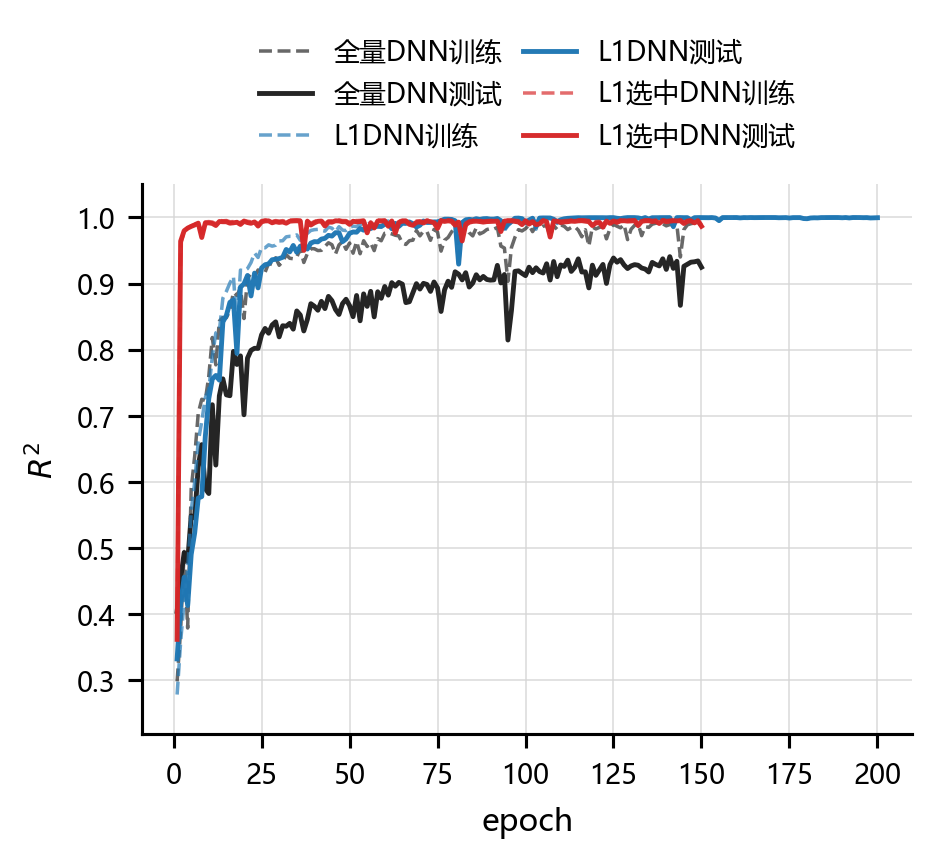
\includegraphics[width=\columnwidth]{redundant_training_congestion_zh.png}\\[-0.2em]
{\scriptsize (a) 日前拥塞价}\\[0.45em]
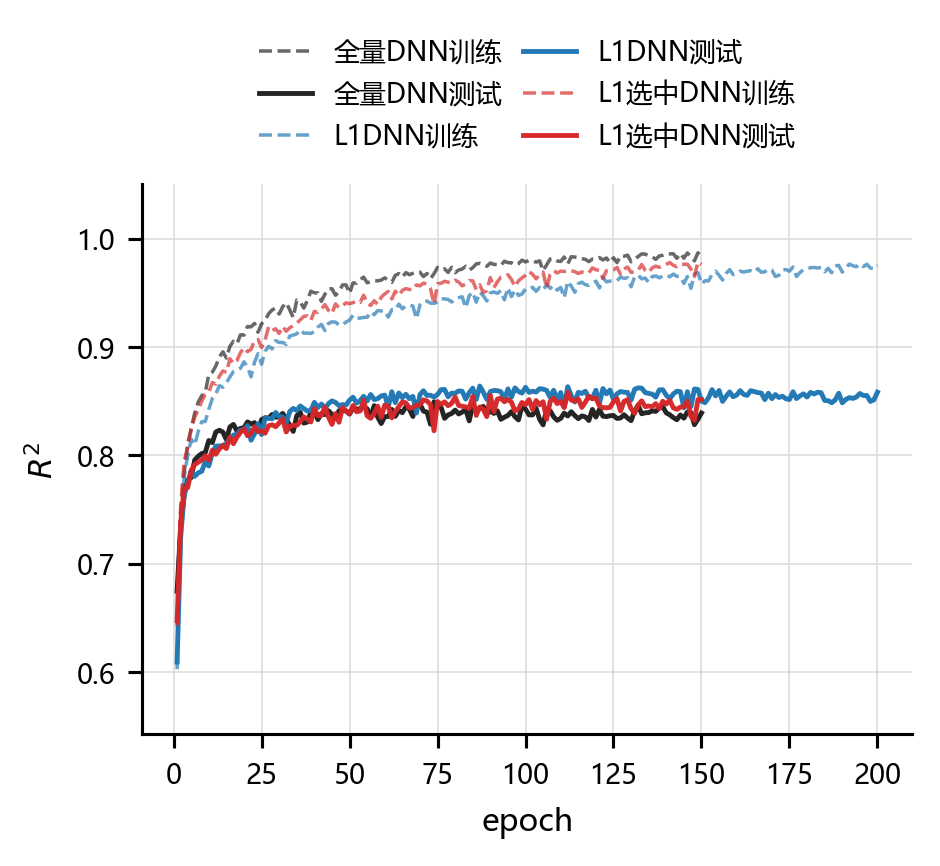
\includegraphics[width=\columnwidth]{redundant_training_primary_zh.png}\\[-0.2em]
{\scriptsize (b) 主备用容量}
\figbicaption{全量字段与 L1 选中特征的训练/测试 $R^2$ 曲线对比}{Comparison of train/test $R^2$ curves between all features and L1-selected features}
\label{fig:redundant_curve}
\end{figure}

\begin{table}[!tbp]
\centering
\scriptsize
\setlength{\tabcolsep}{3pt}
\tabbicaption{冗余噪声解释实验训练曲线统计}{Training-curve statistics for redundant-noise explanation}
\label{tab:noise_curve}
\textbf{(a) 日前拥塞价}\\[-0.2em]
\begin{tabularx}{\columnwidth}{Xrrrr}
\toprule
方法 & 字段数 & Best $R^2$ & epoch & 泛化差距 \\
\midrule
全量 DNN & 69 & 0.9408 & 141 & 0.0621 \\
L1GateDNN & 69 & 1.0000 & 194 & -0.0001 \\
L1 选中特征 DNN & 2 & 0.9954 & 139 & 0.0025 \\
\bottomrule
\end{tabularx}

\vspace{0.4em}
\textbf{(b) 主备用容量}\\[-0.2em]
\begin{tabularx}{\columnwidth}{Xrrrr}
\toprule
方法 & 字段数 & Best $R^2$ & epoch & 泛化差距 \\
\midrule
全量 DNN & 69 & 0.8495 & 74 & 0.1439 \\
L1GateDNN & 69 & 0.8639 & 87 & 0.1170 \\
L1 选中特征 DNN & 35 & 0.8580 & 112 & 0.1247 \\
\bottomrule
\end{tabularx}
\end{table}

\subsubsection{Top-n 递增实验}
为进一步揭示字段数量与推断性能之间的关系，本文按 L1 门控值排名逐步增加输入字段数，记录各组合下的测试 $R^2$。图~\ref{fig:topn_noise} 给出了日前拥塞价和主备用容量两个目标的完整 Top-n 序列结果，其中三角形标记表示 $R^2$ 最高点，方形标记表示全量字段对应的结果。

对于日前拥塞价目标，仅 Top2 字段即达到 0.9954 的测试 $R^2$，Top3 进一步提升至 0.9999，在 Top24 范围内均保持较高水平；然而当字段数增加至 Top32 时，$R^2$ 下降至 0.9851，全量 69 字段的结果仅为 0.9408。对于主备用容量目标，$R^2$ 随字段数从 Top1 到 Top24 逐步提升至 0.8872 的峰值，但继续增加至 Top32 和 Top35 后分别降至 0.8545 和 0.8536，接近全量 DNN 的 0.8495。

上述递增实验揭示了字段数量与推断性能之间的典型非单调关系：当关键字段不足时，模型缺乏必要的信息源，推断能力受限；当字段数量处于合理区间时，核心推断路径被充分激活，推断精度显著提升；而当冗余和弱相关字段继续加入后，输入空间维度增大，过拟合倾向相应上升，导致泛化收益递减甚至出现逆转。实验结果进一步表明，输入字段并非越多越好，在保留主要推断信息的前提下，适度剔除冗余和弱相关字段有助于提升模型的泛化性能。

\begin{figure}[!tbp]
\centering
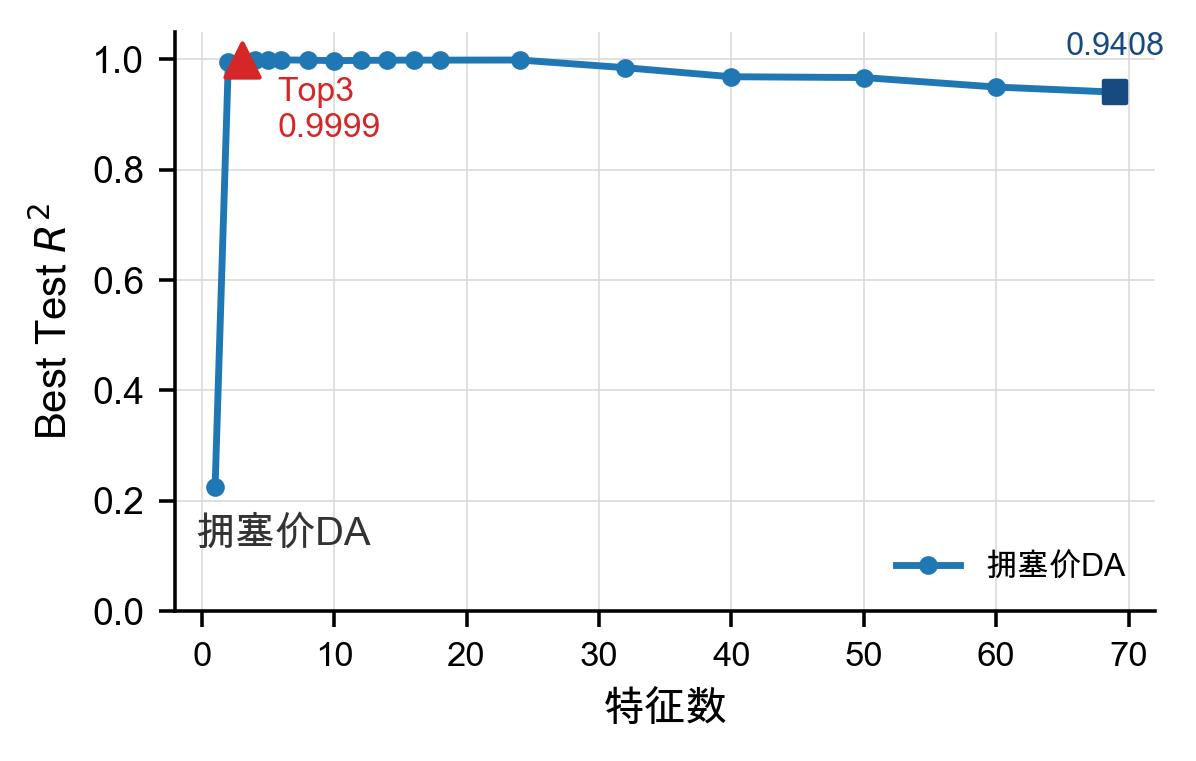
\includegraphics[width=\columnwidth]{topn_congestion_zh.png}\\[-0.2em]
{\scriptsize (a) 日前拥塞价}\\[0.45em]
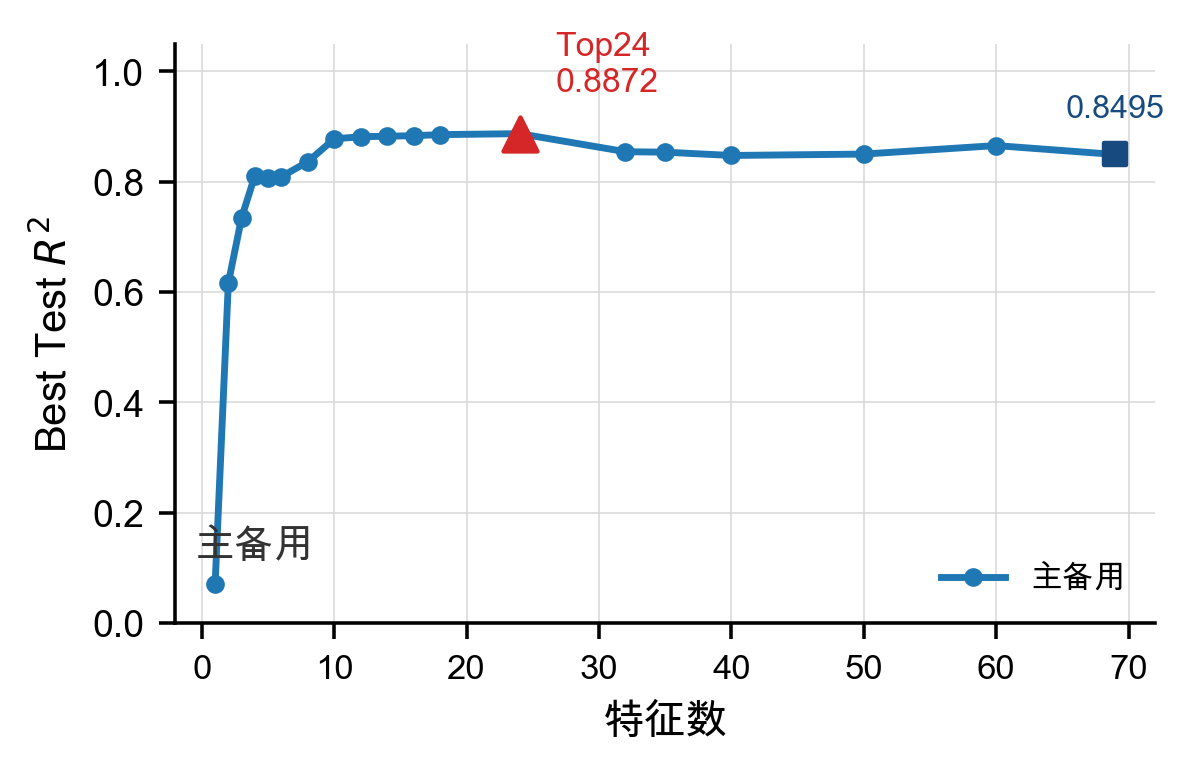
\includegraphics[width=\columnwidth]{topn_primary_zh.png}\\[-0.2em]
{\scriptsize (b) 主备用容量}
\figbicaption{按 L1 门控排名逐步增加字段数的测试 $R^2$ 变化}{Test $R^2$ variation with incrementally added Top-n features ranked by L1 gate values}
\label{fig:topn_noise}
\end{figure}

\section{结论}
本文针对电力数据字段规模大、关联关系复杂以及隐性推断源难以定位的问题，提出了融合多相关性筛选与 L1 门控 DNN 的分析方法。该方法以六类相关性指标进行保守初筛，在 DNN 输入端引入稀疏门控以压缩冗余字段，并通过选中字段再训练验证推断源集合的独立有效性；同时，相关性驱动的改进门控将六类统计证据映射为统一的门控评分，为不同相关性指标对推断源判定的贡献提供了可解释表示。

基于美国 PJM 电力市场 2025 年小时级公开数据的实验结果表明：以净实际交换功率为目标，初筛从 69 个候选字段中保留 55 个字段，L1 门控进一步定位 18 个活跃字段；基于该字段集合再训练的普通 DNN 测试 $R^2$ 为 0.9681，高于全量 69 字段模型的 0.9661，而未选中 51 个字段单独推断的 $R^2$ 仅为 0.7820。在 12 个目标字段上，L1 门控模型以平均 15.5 个字段取得 0.9111 的平均测试 $R^2$，高于全量 DNN 的 0.9031；在 95\% 和 97\% 同预算基线对比中，L1 门控方法也保持最优平均表现。冗余输入影响分析表明，适度压缩弱相关和冗余字段有助于降低过拟合风险，提高模型在测试集上的稳定性。

上述结果说明，所提方法能够在保持目标字段推断能力的同时定位紧凑的关键字段集合，为高维电力数据中的关键变量分析、复杂关联识别和字段间隐含依赖关系挖掘提供了一种有效方法。后续研究将进一步引入多随机种子和跨时间窗口稳定性验证，并将单目标推断分析扩展为多目标关联图谱，以刻画不同目标字段之间的联合推断关系和关联传播路径。

\balance
\begin{thebibliography}{99}
\small
\setlength{\itemsep}{0pt}
\setlength{\parsep}{0pt}
\setlength{\parskip}{0pt}

\bibitem{ref-liu-cps}
刘涛, 田捷, 王杰, 等. 信息物理融合系统的综合安全威胁与防御研究[J]. 自动化学报, 2019, 45(1): 5-24.

LIU Tao, TIAN Jie, WANG Jie, et al. Integrated security threats and defense of cyber-physical systems[J]. Acta Automatica Sinica, 2019, 45(1): 5-24.

\bibitem{ref-ma-pjm}
马子明, 钟海旺, 李竹, 等. 美国电力市场信息披露体系及其对中国的启示[J]. 电力系统自动化, 2017, 41(24): 49-57.

MA Ziming, ZHONG Haiwang, LI Zhu, et al. Information disclosure system in American electricity market and its enlightenment for China[J]. Automation of Electric Power Systems, 2017, 41(24): 49-57.

\bibitem{ref-fan-pjm}
Fan Z, Horger T, Bastian J, et al. An overview of PJM energy market design and development[C]//2008 Third International Conference on Electric Utility Deregulation and Restructuring and Power Technologies. Piscataway: IEEE, 2008: 12-17.

\bibitem{ref-chen-demand}
CHEN Gang, HU Qingchang, WANG Jin, et al. Machine-learning-based electric power forecasting[J]. Sustainability, 2023, 15(14): 11299.

\bibitem{ref-zhu-sharing}
邢汇笛, 龚钢军, 翟明岳, 等. 电力数据共享安全防护与隐私保护综述[J]. 综合智慧能源, 2024, 46(5): 30-40.

XING Huidi, GONG Gangjun, ZHAI Mingyue, et al. Research on security and privacy protection of electric power data sharing[J]. Integrated Intelligent Energy, 2024, 46(5): 30-40.

\bibitem{ref-liu-data-inference}
刘烃, 王子骏, 刘杨, 等. 数据推断: 信息物理融合系统数据泄露威胁范式和防御方法[J]. 中国科学: 信息科学, 2023, 53(11): 2152-2179.

LIU Ting, WANG Zijun, LIU Yang, et al. Data inference: data leakage paradigms and defense methods in cyber-physical systems[J]. Scientia Sinica Informationis, 2023, 53(11): 2152-2179.

\bibitem{ref-sankar}
Sankar L, Rajagopalan S R, Mohajer S, et al. Smart meter privacy: A theoretical framework[J]. IEEE Transactions on Smart Grid, 2013, 4(2): 837-846.

\bibitem{ref-giaconi}
Giaconi G, Gündüz D, Poor H V. Privacy-aware smart metering: Progress and challenges[J]. IEEE Signal Processing Magazine, 2018, 35(6): 59-78.

\bibitem{ref-adewole}
Adewole K S, Torra V. Privacy issues in smart grid data: From energy disaggregation to disclosure risk[C]//International Conference on Database and Expert Systems Applications. Cham: Springer, 2022: 71-84.

\bibitem{ref-zhang-sgcc}
刘家男, 翁健. 智能电网安全研究综述[J]. 信息网络安全, 2016, 16(5): 78-84.

LIU Jianan, WENG Jian. Survey on smart grid security[J]. Netinfo Security, 2016, 16(5): 78-84.

\bibitem{ref-chen-privacy}
邓晓平, 张桂青, 魏庆来, 等. 非侵入式负荷监测综述[J]. 自动化学报, 2022, 48(3): 644-663.

DENG Xiaoping, ZHANG Guiqing, WEI Qinglai, et al. A survey on the non-intrusive load monitoring[J]. Acta Automatica Sinica, 2022, 48(3): 644-663.

\bibitem{ref-lan-load}
严雪颖, 秦川, 鞠平, 等. 负荷功率模型的最优特征选择研究[J]. 电力工程技术, 2021, 40(3): 84-91.

YAN Xueying, QIN Chuan, JU Ping, et al. Optimal feature selection of load power models[J]. Electric Power Engineering Technology, 2021, 40(3): 84-91.

\bibitem{ref-jiao-pv}
Jiao X Y, Sun Y Z, Peng D, et al. Photovoltaic power abnormal data cleaning based on variance change point and correlation analysis[C]//2021 6th International Conference on Power and Renewable Energy (ICPRE). Piscataway: IEEE, 2021: 1140-1145.

\bibitem{ref-deng-load}
Deng X Y, Zhang C K, Peng H, et al. Short-term load forecasting for regional power grids based on correlation analysis and feature extraction[C]//2022 7th Asia Conference on Power and Electrical Engineering (ACPEE). Piscataway: IEEE, 2022: 1081-1085.

\bibitem{ref-szekely-dcorr}
Székely G J, Rizzo M L, Bakirov N K. Measuring and testing dependence by correlation of distances[J]. The Annals of Statistics, 2007, 35(6): 2769-2794.

\bibitem{ref-reshef-mic}
Reshef D N, Reshef Y A, Finucane H K, et al. Detecting novel associations in large data sets[J]. Science, 2011, 334(6062): 1518-1524.

\bibitem{ref-xing-micdnn}
Xing Z Y, Wang Z J, Feng J L, et al. MIC-DNN: data-driven correlation analysis framework for power data[C]//2025 40th Youth Academic Annual Conference of Chinese Association of Automation (YAC). Piscataway: IEEE, 2025: 2969-2974.

\bibitem{ref-lecun-deep}
LeCun Y, Bengio Y, Hinton G. Deep learning[J]. Nature, 2015, 521(7553): 436-444.

\bibitem{ref-goodfellow-deep}
Goodfellow I, Bengio Y, Courville A. Deep learning[M]. Cambridge: MIT Press, 2016.

\bibitem{ref-breiman-rf}
Breiman L. Random forests[J]. Machine Learning, 2001, 45(1): 5-32.

\bibitem{ref-chen-xgboost}
Chen T, Guestrin C. XGBoost: A scalable tree boosting system[C]//Proceedings of the 22nd ACM SIGKDD International Conference on Knowledge Discovery and Data Mining. New York: ACM, 2016: 785-794.

\bibitem{ref-wang-meter}
Wang Y, Chen Q, Hong T, et al. Review of smart meter data analytics: Applications, methodologies, and challenges[J]. IEEE Transactions on Smart Grid, 2019, 10(3): 3125-3148.

\bibitem{ref-tibshirani-lasso}
Tibshirani R. Regression shrinkage and selection via the lasso[J]. Journal of the Royal Statistical Society: Series B, 1996, 58(1): 267-288.

\bibitem{ref-zou-enet}
Zou H, Hastie T. Regularization and variable selection via the elastic net[J]. Journal of the Royal Statistical Society: Series B, 2005, 67(2): 301-320.

\bibitem{ref-pearson}
Pearson K. Notes on regression and inheritance in the case of two parents[J]. Proceedings of the Royal Society of London, 1895, 58: 240-242.

\bibitem{ref-spearman}
Spearman C. The proof and measurement of association between two things[J]. The American Journal of Psychology, 1904, 15(1): 72-101.

\bibitem{ref-kendall}
Kendall M G. A new measure of rank correlation[J]. Biometrika, 1938, 30(1/2): 81-93.

\bibitem{ref-cover-info}
Cover T M, Thomas J A. Elements of information theory[M]. 2nd ed. Hoboken: John Wiley \& Sons, 2006.

\bibitem{ref-gretton-hsic}
Gretton A, Bousquet O, Smola A, et al. Measuring statistical dependence with Hilbert-Schmidt norms[C]//Algorithmic Learning Theory. Berlin: Springer, 2005: 63-77.

\bibitem{ref-pjm-dataminer}
PJM Interconnection. PJM Data Miner 2[EB/OL]. [2025-05-01]. https://dataminer2.pjm.com.

\bibitem{ref-kingma-adam}
Kingma D P, Ba J. Adam: A method for stochastic optimization[C]//International Conference on Learning Representations. San Diego: ICLR, 2015.
\end{thebibliography}

\section*{收稿日期与作者简介}
\noindent\textbf{收稿日期：}20XX-XX-XX

\noindent\textbf{作者简介：}\par
\noindent 杜浩存（出生年），男，研究方向为电力数据关联分析、信息物理系统安全与机器学习，邮箱：待补充。

\end{document}
